%%
%% This is file `sample-acmlarge.tex',
%% generated with the docstrip utility.
%%
%% The original source files were:
%%
%% samples.dtx  (with options: `all,journal,bibtex,acmlarge')
%% 
%% IMPORTANT NOTICE:
%% 
%% For the copyright see the source file.
%% 
%% Any modified versions of this file must be renamed
%% with new filenames distinct from sample-acmlarge.tex.
%% 
%% For distribution of the original source see the terms
%% for copying and modification in the file samples.dtx.
%% 
%% This generated file may be distributed as long as the
%% original source files, as listed above, are part of the
%% same distribution. (The sources need not necessarily be
%% in the same archive or directory.)
%%
%%
%% Commands for TeXCount
%TC:macro \cite [option:text,text]
%TC:macro \citep [option:text,text]
%TC:macro \citet [option:text,text]
%TC:envir table 0 1
%TC:envir table* 0 1
%TC:envir tabular [ignore] word
%TC:envir displaymath 0 word
%TC:envir math 0 word
%TC:envir comment 0 0
%%

%% For submission and review of your manuscript please change the
%% command to \documentclass[manuscript, screen, review]{acmart}.
%%
%% When submitting camera ready or to TAPS, please change the command
%% to \documentclass[sigconf]{acmart} or whichever template is required
%% for your publication.
%%
%%
\documentclass[manuscript,review,anonymous]{acmart}
%\documentclass[acmlarge,review=true, anonymous=false,authordraft]{acmart}
%%

\usepackage{fontawesome}
\usepackage{float}
\usepackage{tabularx}
\usepackage{dcolumn} %Aligning numbers by decimal points in table columns
\newcolumntype{d}[1]{D{.}{.}{#1}}
\usepackage{float}
\usepackage{subcaption}
\usepackage{makecell}
 \usepackage{threeparttable} 
\usepackage{todonotes}
\usepackage[normalem]{ulem}
\usepackage{tikz}
% \usepackage{amssymb}

\newcommand{\blackcircled}[1]{%
  \tikz[baseline=(char.base)]{
    \node[circle,fill=black,text=white,inner sep=.5pt] (char) {\textbf{\sffamily #1}};
  }%
}

\useunder{\uline}{\ul}{}
\let\xtodo\todo
\renewcommand{\todo}[1]{\xtodo[inline,color=green!50]{#1}}
% Special TODOs added by review pass:
%   \todoredundant — content repeated elsewhere in the manuscript
%   \todoshort     — verbose passage; a shorter rewrite is provided beneath
%   \todoterm      — inconsistent terminology / naming / capitalization
\newcommand{\todoredundant}[1]{\xtodo[inline,color=red!35]{\textbf{REDUNDANT:} #1}}
\newcommand{\todoshort}[1]{\xtodo[inline,color=cyan!30]{\textbf{SHORTER:} #1}}
\newcommand{\todoterm}[1]{\xtodo[inline,color=yellow!50]{\textbf{TERMINOLOGY:} #1}}

\definecolor{colortodo}{rgb}{0.9, 0.6, 0}    
\definecolor{colordaniel}{rgb}{0, 0.7, 0.35}
\definecolor{colorthomas}{rgb}{0.2, 0.4, 0.8}
\definecolor{colorrobin}{rgb}{0.2, 0.8, 0.9}
\definecolor{colordaniela}{rgb}{0.8, 0.2, 0.7}
\definecolor{colornotfinal}{rgb}{0.95, 0.2, 0.2} 
\definecolor{colorlev}{rgb}{0.4, 0.2, 0.2}

\newcommand{\tba}{\textcolor{colortodo}
{\faExclamationTriangle\ \texttt{TBA}}}

\newcommand{\nf}[1]{\textcolor{colornotfinal}{#1}} % not final

\newcommand{\thomas}[1]{\textcolor{colorthomas}{\textbf{\faComment~Thomas:} #1}}

\newcommand{\lev}[1]{\textcolor{colorlev}{\textbf{\faComment~Lev:} #1}}

\newcommand{\daniela}[1]{\textcolor{colordaniela}{\textbf{\faComment~Daniela:} #1}}

\newcommand{\daniel}[1]{\textcolor{colordaniel}{\textbf{\faComment~Daniel:} #1}}

\newcommand{\robin}[1]{\textcolor{colorrobin}{\textbf{\faComment~Robin:} #1}}

\newcommand{\todolist}[1]{%
  \noindent\textcolor{colortodo}{\rule{\linewidth}{0.2pt}}\\[0.2em]%
  \noindent\textcolor{colortodo}{\faWrench~\textbf{TODO:} #1} \\
  \noindent\textcolor{colortodo}{\rule{\linewidth}{0.2pt}}\\
}

\newif\ifnewtext
\newtexttrue        %  <-- \newtextfalse for the submission build
\definecolor{colornew}{rgb}{0.75, 0.05, 0.05}
\newcommand{\new}[1]{\ifnewtext\textcolor{colornew}{#1}\else#1\fi}
% \newenvironment{newblock}{\ifnewtext\color{colornew}\fi\ignorespaces}{}
% Marking text *inside a section heading*: \texorpdfstring keeps the colour out
% of the PDF bookmark, which hyperref cannot typeset.
\newcommand{\newh}[1]{\texorpdfstring{\new{#1}}{#1}}
% Floats do not reliably inherit \color from the surrounding newblock, so a
% table that is wholly new opens with \newfloatcolor.
\newcommand{\newfloatcolor}{\ifnewtext\color{colornew}\fi}

%% \BibTeX command to typeset BibTeX logo in the docs
\AtBeginDocument{%
  \providecommand\BibTeX{{%
    Bib\TeX}}}

%% Rights management information.  This information is sent to you
%% when you complete the rights form.  These commands have SAMPLE
%% values in them; it is your responsibility as an author to replace
%% the commands and values with those provided to you when you
%% complete the rights form.
\setcopyright{acmlicensed}
\copyrightyear{2027}
\acmYear{2027}
\acmDOI{}
%% These commands are for a PROCEEDINGS abstract or paper.
\acmConference[CHI '27]{CHI Conference on Human Factors in Computing Systems}{May 10-14, 2027}{Pittsburgh, PA}
%%
%%  Uncomment \acmBooktitle if the title of the proceedings is different
%%  from ``Proceedings of ...''!
%%
%%\acmBooktitle{Woodstock '18: ACM Symposium on Neural Gaze Detection,
%%  June 03--05, 2018, Woodstock, NY}
\acmISBN{}

%%
%% Submission ID.
%% Use this when submitting an article to a sponsored event. You'll
%% receive a unique submission ID from the organizers
%% of the event, and this ID should be used as the parameter to this command.
%%\acmSubmissionID{123-A56-BU3}

%%
%% For managing citations, it is recommended to use bibliography
%% files in BibTeX format.
%%
%% You can then either use BibTeX with the ACM-Reference-Format style,
%% or BibLaTeX with the acmnumeric or acmauthoryear sytles, that include
%% support for advanced citation of software artefact from the
%% biblatex-software package, also separately available on CTAN.
%%
%% Look at the sample-*-biblatex.tex files for templates showcasing
%% the biblatex styles.
%%

%%
%% The majority of ACM publications use numbered citations and
%% references.  The command \citestyle{authoryear} switches to the
%% "author year" style.
%%
%% If you are preparing content for an event
%% sponsored by ACM SIGGRAPH, you must use the "author year" style of
%% citations and references.
%% Uncommenting
%% the next command will enable that style.
%%\citestyle{acmauthoryear}


%%
%% end of the preamble, start of the body of the document source.
\begin{document}




%%
%% The "title" command has an optional parameter,
%% allowing the author to define a "short title" to be used in page headers.
\title{Explaining Too Much? Understanding How Large Language Model Reasoning Traces Influence Performance and Metacognition}

%%
%% The "author" command and its associated commands are used to define
%% the authors and their affiliations.
%% Of note is the shared affiliation of the first two authors, and the
%% "authornote" and "authornotemark" commands
%% used to denote shared contribution to the research.


\author{Daniela Fernandes}
\email{daniela.dasilvafernandes@aalto.fi}
\orcid{0009-0006-1332-7485}
\affiliation{%
  \institution{Aalto University}
  \city{Espoo}
  \country{Finland}
}

\author{Daniel Buschek}
\email{daniel.buschek@uni-bayreuth.de}
\orcid{0000-0002-0013-715X}
\affiliation{%
  \institution{University of Bayreuth}
  \city{Bayreuth}
  \country{Germany}
}

\author{Lev Tankelevitch}
\email{levt@microsoft.com}
\orcid{0000-0003-1286-5194}
\affiliation{%
  \institution{Microsoft Research Cambridge}
  \city{Cambridge}
  \country{United Kingdom}
}


\author{Thomas Kosch}
\email{thomas.kosch@hu-berlin.de}
\orcid{0000-0001-6300-9035}
\affiliation{%
  \institution{HU Berlin}
  \city{Berlin}
  \country{Germany}
}


\author{Robin Welsch}
\email{robin.welsch@aalto.fi}
\orcid{0000-0002-7255-7890}
\affiliation{%
  \institution{Aalto University}
  \city{Espoo}
  \country{Finland}
}


%%
%% By default, the full list of authors will be used in the page
%% headers. Often, this list is too long, and will overlap
%% other information printed in the page headers. This command allows
%% the author to define a more concise list
%% of authors' names for this purpose.
\renewcommand{\shortauthors}{Fernandes et al.}

%%
%% The abstract is a short summary of the work to be presented in the
%% article.
\begin{abstract}
%\todo{What is the specific problem addressed?}
%\todo{What have you done?}
%\todo{What did you find out?}
%\todo{What are the implications on a larger scale?}
%Generative AI is increasingly embedded in reasoning-, learning-, and creativity-oriented workflows. In parallel, 
%Large Language Model (LLM) interfaces are becoming more verbose, increasingly exposing \textit{reasoning traces} alongside final answers. 

Large Language Model interfaces are increasingly verbose, exposing intermediate reasoning traces alongside final answers. Traces are framed as transparency mechanisms, yet it is unclear how people use them to solve problems. We report two between-subjects studies. Study 1 is a preregistered between-subjects experiment (N = 556) in which participants solved ten LSAT-style reasoning problems under one of three conditions: an \textit{Answer-only} baseline, a \textit{Full-trace} revealed before the answer, and a \textit{Summary-trace} presented alongside the answer. Summaries preserved task performance at the no-trace baseline while significantly elevating trust and hedonic appeal, establishing that trace exposure shifts subjective appraisal of the interaction without bringing performance benefits. Under an open-weight reasoning model exposing verbose intermediate output, full traces additionally impaired performance relative to the answer-only baseline. Across all conditions, participants substantially overestimated their performance, and no trace format supported calibrated self-evaluation. Further analysis indicates that hedonic appeal, not trust, carries the indirect path to overestimation, consistent with a processing-fluency account. Because trace format was confounded with model identity in Study 1, Control Study (N = 163) holds the model constant across all three conditions and varies only the length of the reasoning displayed: an \textit{Answer-only} baseline, a \textit{Short-trace}, and a \textit{Long-trace}. The performance impairment did not reappear, and overestimation persisted at every trace length, indicating that neither effect is a property of trace verbosity. Reasoning traces are best understood as user-facing interface artifacts rather than transparent windows into model cognition, and calibration is unlikely to emerge from the traces themselves and may rather best be scaffolded by interactions that elicit users' own reasoning first.


% Large Language Model interfaces are increasingly verbose, exposing intermediate reasoning traces alongside final answers. Traces are framed as transparency mechanisms, yet it is unclear how people use them to solve problems.  We report a preregistered between-subjects study ($N=559$) in which participants solved ten Law School Admission Test-style reasoning problems under one of three conditions: an \textit{Answer-only} baseline, a \textit{Full-trace} revealed before the answer, and a \textit{Summary-Trace} presented alongside the answer.%
% Full traces did not improve task performance; participants in the \textit{Full-trace} condition performed significantly worse than those given the model's answer alone, while summaries merely preserved performance at the no-trace baseline. Across all conditions, participants substantially overestimated their performance, with the largest miscalibration under full traces. Despite delivering no performance benefit, both trace conditions were rated as more trustworthy.%
% We argue that reasoning traces are best understood as user-facing interface artifacts rather than as transparent windows into the model's inner workings, and that calibration is unlikely to emerge from the traces themselves. By empirically contrasting trace designs, we uncover mechanisms through which traces shape HAI and derive design principles that balance effectiveness, calibration, user experience, and usability.%



% Large Language Model (LLM) interfaces are increasingly verbose, exposing intermediate reasoning traces alongside final answers. 
% While traces are framed as mechanisms for transparency, prior work suggests that fluent justifications can induce a sense of understanding and shift how people monitor their own decisions. How reasoning traces shape user metacognition in Human–AI Interaction (HAI), however, remains poorly understood.
% %While traces are often framed as a mechanism for transparency and user sensemaking, it remains unclear whether they reliably support users’ decision-making and task performance. Prior work on explanation interfaces points to additional risks. High-verbosity outputs may induce a sense of understanding, increase overreliance and shift how people monitor their own decisions. Thus, a key open question is how reasoning traces shape metacognition in Human-AI Interaction (HAI) and calibrate reliance on AI.
% We report a preregistered between-subjects study ($N=559$) in which participants solved ten Law School Admission Test-style reasoning problems with AI assistance and were exposed to different shapes of reasoning traces under one of three conditions: \textit{Answer-only} baseline (C1), \textit{Full reasoning traces} revealed before the answer (C2), and a \textit{Summary of reasoning traces} presented alongside the answer (C3).  Full traces did not improve task performance. Participants in the Full-trace condition performed significantly worse than those given only the model's answer, while summarized traces merely preserved performance at the no-trace baseline. Across all three conditions, participants substantially overestimated their performance, and this miscalibration was largest under full traces. Despite delivering no performance or calibration benefit, both trace conditions were rated as more trustworthy. We argue that reasoning traces are best understood as user-facing interface artifacts rather than transparent windows into the inner working of the model, and that calibration is unlikely to emerge from the trace itself. By systematically contrasting reasoning trace designs, we uncover mechanisms through which reasoning traces influence human–AI interaction and derive design principles that balance effectiveness, calibration, user experience and usability.

%Large language model (LLM) interfaces increasingly expose their intermediate reasoning traces alongside final outputs. Yet it remains unclear whether such traces help users make better decisions, increase overconfidence, or improve the calibration of metacognitive judgments. We report a between-subjects experiment in which participants completed logical reasoning tasks under three interface conditions: (1) no reasoning trace (final answer only), (2) full reasoning trace revealed before the final answer, and (3) a concise summary of the reasoning plus the final answer. We examine what benefits or drawbacks these formats have for task accuracy and efficiency, how they shape metacognitive sensitivity (confidence–accuracy alignment) and trust calibration, and why users encounter distinct usability and user-experience trade-offs across designs. By systematically contrasting reasoning trace designs, we uncover mechanisms through which reasoning traces influence human–AI interaction and derive design principles that balance effectiveness, calibration, user experience and usability.
\end{abstract}

%%
%% The code below is generated by the tool at http://dl.acm.org/ccs.cfm.
%% Please copy and paste the code instead of the example below.
%%
\begin{CCSXML}
<ccs2012>
    <concept>
        <concept_id>10003120.10003121.10003128</concept_id>
        <concept_desc>Human-centered computing~Human-Computer Interaction (HCI)</concept_desc>
        <concept_significance>300</concept_significance>
    </concept>
 </ccs2012>
\end{CCSXML}
\ccsdesc[500]{Human-centered computing~Human computer interaction (HCI)}

%%
%% Keywords. The author(s) should pick words that accurately describe
%% the work being presented. Separate the keywords with commas.
\keywords{Metacognition, Reasoning Traces, Large Language Models, Overconfidence}

\received{20 February 2007}
\received[revised]{12 March 2009}
\received[accepted]{5 June 2009}

%%
%% This command processes the author and affiliation and title
%% information and builds the first part of the formatted document.
\maketitle


\todo{Disclaimer: Draft is still very LLMy}

\section{Introduction}

Large Language Models (LLMs) are becoming increasingly verbose, with users now exposed not only to final outputs but also to intermediate ``reasoning traces'', chain-of-thought-style outputs that resemble the model's inner workings \cite{barez2025chain}. Showing reasoning traces promises transparency. Reasoning traces are meant to help users make sense of AI answers and scaffold complex workflows \cite{6645235,anthropic2025extended,openai2024learning,openai2025monitorability}. As a result, AI Providers explicitly market reasoning traces as tools for transparency \cite{lindsey2025biology}, while the generation of traces increases the amount of spent tokens compared to a direct answer \cite{sui2025stop, anthropic2025extended}. The design question is thus whether exposing reasoning traces provides the transparency providers claim, with benefits for their users. As such, users can make more informed decisions about the generated output when viewing the reasoning traces.

However, prior research in eXplainable AI (XAI) and Human-Computer Interaction (HCI) reports mixed findings on the efficacy of reasoning traces. High verbosity of LLM output can induce an illusion of understanding (e.g., illusions of knowledge \cite{fisher2021harder}), and fluent justifications may lead users toward overreliance even when the underlying conclusion is wrong \cite{10.1145/3397481.3450639, 10.1145/3449287}. Moreover, a model's ``chain-of-thought'' is not always faithful to its intermediate steps and can function as a polished, but misleading, justification \cite{10.5555/3666122.3669397,lindsey2025biology, barez2025chain}. At the same time, while AI has the potential to improve task performance \cite{10.1145/3411764.3445717, steyvers_bayesian_2022,zulfikar_memoro_2024}, users tend to believe they perform better when assisted by AI \cite{FERNANDES2026108779, kloft2023ai, villa2023placebo, kosch2023placebo} and struggle to align confidence with correctness. Previous research shows that the core challenge of understanding not only how people can make better decisions with AI, but how AI interfaces shape \textit{metacognition}, that is, users' ability to monitor and evaluate their own decisions and regulate reliance during interaction with AI.%

%Recent interpretability work further explores this: internal model computations and chain-of-thought outputs can diverge, and what the model outputs as a ``reasoning trace'' may not faithfully represent how it actually arrived at its answer \cite{lindsey2025biology, barez2025chain}. %\footnote{Recent interpretability work further explores this: internal model computations and chain-of-thought outputs can diverge, and what the model outputs as a ``reasoning trace'' may not faithfully represent how it actually arrived at its answer \cite{lindsey2025biology, barez2025chain}. For the purposes of this study, we introduce a different reframing. Rather than treating traces as ground-truth windows into model cognition, we treat them as user-facing interface artifacts, e.g., a type of XAI output that users respond to regardless of its internal validity. The relevant question for our study is not whether the trace accurately reflects the model's computation, but whether and how it shapes the user's metacognitive processes. This framing is consistent with the XAI literature's distinction between proxy explanations and faithful explanations \cite{barez2025chain, jacovi-goldberg-2020-towards, 10.5555/3666122.3669397}, and it positions the faithfulness problem as a further design risk: users may calibrate their reliance on outputs that are themselves unreliable representations of model "thinking", amplifying the metacognitive consequences.}

%At the same time, while AI has the potential to improve task performance \cite{10.1145/3411764.3445717, steyvers_bayesian_2022,zulfikar_memoro_2024}, users often believe they perform better when assisted by AI \cite{FERNANDES2026108779, kloft2023ai, villa2023placebo} and struggle to align confidence with correctness. This highlights the core challenge of understanding not only how people can make better decisions with AI, but how AI interfaces shape \textit{metacognition}, that is, users' ability to monitor and evaluate their own decisions and regulate reliance during interaction with AI.%

In this paper, we investigate how the shape of reasoning traces affects performance and metacognition in human-AI reasoning contexts: %(in our study, we treat reasoning traces as a form of explainability for LLMs).
Specifically, we ask (1) what the benefits and drawbacks of different reasoning-trace formats are, (2) how these formats affect task performance, (3) how they shape metacognition, and (4) whether they can support calibrated reliance on AI. 

To address these questions, we present findings from a preregistered between-subjects experiment (N = 556) in which participants solved ten LSAT-style logical reasoning problems with AI assistance under one of three interface conditions that span the practically relevant design space for exposing model reasoning:


\begin{itemize}
    \item \textit{Answer-only} condition (N = 187): An answer-only baseline that reflects early LLM interfaces.
    \item \textit{Full-trace} condition (N = 181): A full reasoning trace shown before the model's final answer, which remained hidden behind a button press. This ensured that participants engaged with the trace itself rather than the verdict, and mirrored the verbose outputs of current open-weight reasoning models.
    \item \textit{Summary-trace} condition (N = 188): A summary of reasoning traces presented together with the answer, of the kind now adopted by several commercial systems (see \cite{openai2024learning, anthropic2025extended}).
\end{itemize}

These three formats capture the dominant ways in which reasoning is currently surfaced to users and allow us to control verbosity in our study. By isolating the \textit{content} of the trace from how it is revealed, we can ask whether traces help, hurt, or need to be calibrated, and at what level of verbosity, if any, they support metacognitive accuracy rather than merely inflating the appearance of understanding. LSAT-style reasoning has been established as a robust measure of both performance and metacognition \cite{vaccaro2024combinations}, has been used in prior human-AI interaction research \cite{FERNANDES2026108779}, and serves as a benchmark for evaluating LLMs \cite{katz2024gpt}. 


Across five outcomes (task performance, metacognitive accuracy, task load, trust, and usability), our results converge on a consistent dissociation: Trace exposure shifts subjective appraisal of the interaction without bringing performance benefits. Summary traces preserved task performance at the no-trace baseline while significantly elevating trust and hedonic appeal  which provides a contrast in which the underlying LLM model was held constant (GPT-5). Under an open-weight reasoning model exposing verbose intermediate output (GPT-oss-20b), full traces additionally impaired performance relative to the \textit{Answer-only} baseline. Across all three conditions, participants substantially overestimated their performance, and no trace format supported calibrated self-evaluation. However, overestimation was largest under \textit{Full-trace}. A mediation analysis indicates that hedonic appeal, not trust, carries the indirect path to overestimation, consistent with a processing-fluency account of metacognitive misattribution.

Because no frontier model exposes its full reasoning, the \textit{Full-trace} condition required a different model than the other two, confounding trace format with model identity. A second, smaller study (N = 163, reported in the appendix) therefore holds the model constant and varies only the length of the reasoning displayed; we summarize its design and results.

Our contributions are threefold. First, we provide a \textit{controlled comparison of reasoning-trace formats} in terms of cognitive and metacognitive performance. %We isolate verbosity as a design dimension and show that summarized traces preserve performance without improving calibration while elevating subjective appraisal of the interaction.
Second, we show that \textit{summaries preserve performance without improving calibration} while raising trust and hedonic appeal, and that under an open-weight verbose-trace regime, full traces additionally impair performance and produce the largest overestimation gap. This implies that calibration is unlikely to emerge from the trace itself, regardless of verbosity.
Third, we translate these findings into \textit{concrete design directions} for trace-based LLM interfaces: We argue that reasoning traces are best understood as user-facing interface artifacts rather than windows into model cognition. Metacognitive support must instead be scaffolded by interactions that elicit users' own reasoning before exposing the model's reasoning traces or answer.

% Across five outcomes (task performance, metacognitive accuracy, task load, trust, and usability), our results converge on the pattern that more reasoning-trace output did not improve task performance. Participants in the \textit{Full-trace} condition performed worse than those in the \textit{Answer-only} condition ($M$=5.46 \textit{vs}. $M$=6.18 items correct) while summarized traces merely preserved performance at the no-trace baseline. Across all three conditions, participants substantially overestimated their performance, and this miscalibration was largest under the \textit{Full-trace} condition. Despite these costs, both trace conditions (\textit{Full-trace} and \textit{Summary-trace}) were rated as more trustworthy and as offering a better user experience than the \textit{Answer-only} baseline, even though they delivered no performance or calibration benefit.


% %Yet trace conditions were rated as more trustworthy and as offering a better user experience than the answer-only baseline, despite delivering no performance or calibration benefit.


% % To address this gap, we present findings from a between-subjects experiment on the Law School Admission Test (LSAT)-style reasoning tasks, comparing three interface designs that vary the form of reasoning traces (\textit{Answer-only} (C1), \textit{Full reasoning traces} (C2), or a \textit{Summary of reasoning traces} (C3)). The LSAT-reasoning part has shown to be a good performance measure and metacognition \cite{NATURE HUMAN BEHAVIOR PAPER} that has been used in HAI research \cite{FERNANDES2026108779} but also for benchmarking AI models \cite{}. We report on metacognitive accuracy, sensitivity, and trust calibration alongside performance and user experience.


% Our contributions are threefold. First, we provide a \textit{controlled comparison of reasoning-trace formats} in terms of cognitive and metacognitive performance. We isolate verbosity as a single design dimension, showing that more verbose traces can reduce performance rather than support it.

% Second, we show that \textit{full reasoning traces impair cognitive performance} relative to an answer-only baseline and produce the largest overestimation gap, whereas summaries preserve performance without improving metacognitive accuracy across conditions. This implies that calibration is unlikely to emerge from the trace itself. %which implies that more reasoning output does not yield better calibration.

% Third, we translate these findings into \textit{concrete design directions} for trace-based LLM interfaces: We argue that reasoning traces are best understood as user-facing interface artifacts rather than windows into model cognition. Thus, metacognitive support must instead be scaffolded by interactions that elicit users' own reasoning before exposing the model's reasoning traces.
%and must instead be scaffolded by interactions that elicit the user's own reasoning before exposing the model's reasoning traces.

% Large Language Models are becoming increasingly verbose, with users now being exposed to both the final output and the model's intermediate "reasoning traces" (chain-of-thought style outputs). 
% Reasoning traces carry the promise of transparency, improving users' understanding of the AI's output and scaffolding complex workflows. However, prior research on XAI and HCI report mixed findings. High verbosity might induce a sense of understanding (e.g., illusions of knowledge, \cite{}), influencing users towards overreliance on AI due to the apparent fluency. Moreover, the model's chain of thought is not always faithful to intermediate steps, occasionally serving as polished but misleading justifications

% Despite prior work showing AI has the potential to increase task performance \cite{}, users believe they perform better when assisted by AI \cite{}, failing to align confidence and correctness. We thus face the core challenge of understanding not only how people can make better decisions when using AI but also how such interfaces shape metacognition (e.g., the ability to monitor and evaluate one's own decisions).

% We thus attempt to clarify the effects of reasoning traces on metacognition, more specifically, what are the benefits and drawbacks of different reasoning trace formats, what are the effects on task performance and decision accuracy, how it affects metacognitive sensitivity and if it can help regulate and calibrate reliance in AI. We aim to observe if users experience different usability and user-experience trade-offs across formats.


% Our contributions are threefold. We provide a systematic comparison of reasoning-trace formats in a controlled study of human-AI interaction; we report empirical insights on metacognitive accuracy, sensitivity, and trust calibration alongside performance and user experience; and we clarify actionable design principles (\textit{Tools for Thought strategies}) for calibration-aware interfaces to LLM reasoning traces.
%We discuss how future work aims to clarify actionable design principles for calibration-aware interfaces for LLM reasoning traces and highlight design principles to contribute to more effective explanation interfaces.


% \textbf{Research Questions}: \daniela{needs to be merged into text}

% RQ1 (Metacognitive accuracy):
% Do summarized reasoning traces improve users’ awareness of their own performance, relative to full traces and to no traces?
% %H1: $C3 \gt C2 \gt C1$; reduced overestimation. Measures: bias (perceived − actual),  Sensitivity: trial-level confidence–accuracy AUC.

% RQ2 (Cognitive load): Do full reasoning traces increase cognitive load compared to summaries or no traces?
% %H2:$C2 \gt C1$ and $C2 \gt C3$; expect $C3 \gtrsim C1$. Measures: NASA-TLX (raw)

% RQ3 (Trust and confidence): Do full reasoning traces elevate users’ confidence and trust in the AI relative to summaries and no traces?
% %H3: $C2 \geq C3 \gt C1$. Measures: mean confidence (0–100), XAI Trust scale.

% RQ4 (Objective performance): Do reasoning traces (full or summary) improve task accuracy relative to answer-only?
% %H4: $ C2 \geq C3 \gt C1$. Measure: accuracy (proportion correct across items).

% RQ5: When using AI on reasoning tasks, are people more likely to prefer a summary of the reasoning traces as compared to being exposed to full reasoning traces? 
% % H5: $C1\geq C3\gt C2$ (System Usability Scale)





\section{Related Work}

In this section, we focus on the role of metacognitive processes in human cognition and human–AI interaction. We first introduce central concepts of human metacognition and examine how mechanisms such as self-monitoring and evaluation influence problem-solving, learning, and decision-making. We then consider how these processes are affected when people collaborate with AI systems, highlighting both opportunities and risks for cognitive performance and user judgment. Finally, we introduce key concepts related to reasoning traces and AI explanations, which aim to increase transparency but may also introduce new challenges for calibration and usability.

\subsection{Metacognition and Human Reasoning}\label{sec:human_metacognition}
Metacognition refers to the processes by which people monitor, plan, and evaluate their own thinking \cite{fleming2024metacognition}. These processes are essential for complex problem-solving, learning, and optimizing behavior. Two primary constructs have been emphasized in psychological research: metacognitive accuracy and metacognitive sensitivity.

\textit{Metacognitive accuracy} describes how closely individuals' self-evaluations align with their actual performance \cite{fleming2024metacognition, colombatto2023illusions}. High accuracy allows people to recognize their limitations and make informed adjustments, such as seeking more information, revising a strategy, or making a conservative choice. Accuracy can be further decomposed into bias (systematic over- or underestimation) and noise (random fluctuations) \cite{fiedler2019metacognition}.

\textit{Metacognitive sensitivity} refers to the ability to discriminate between correct and incorrect judgments, often measured through confidence ratings after the decision \cite{fleming2024metacognition}. High metacognitive sensitivity entails that an individual's confidence ratings accurately reflect their performance: high confidence corresponds to correct judgments, and low confidence to incorrect ones.

Both constructs show substantial individual differences \cite{kelemen2000individual, ackerman2017meta} and are affected by external aids. People often misattribute externally generated information to themselves \cite{johnson_source_1993, Zindulka2026AIMemoryGap}, and reading fluent explanations inflates perceived understanding even when comprehension has not actually improved \cite{fisher2021harder}. These findings establish an underlying expectation that any system that provides articulate external reasoning may shift users' self-evaluations, regardless of whether it improves their actual performance.

%Research shows substantial individual differences in metacognitive ability \cite{kelemen2000individual; ackerman2017meta}. While some individuals monitor and adjust their performance effectively, others fail to do so, particularly when overreliance on external aids undermines self-evaluation.

%Design research has begun to apply these insights to interactive systems. Tailoring AI interactions to users’ metacognitive processes, for example by crafting prompts, decomposing complex tasks, or allowing users to edit AI outputs, can enhance performance, mitigate errors, and foster a sense of agency \cite{tankelevitch2023metacognitive; draxlerghost24}. Similarly, small interface modifications such as introducing natural language uncertainty cues (e.g., "I am not sure, but...") can reduce overreliance and improve accuracy \cite{kim2024m}. However, it can also lead to deskilling, as it has been seen when generative AI improves short-term performance but undermines learning and long-term ability \cite{bastani2024generative; rafner2022deskilling; Kobiella2024}. Designing human–AI systems that explicitly support metacognition is therefore crucial to reduce deskilling while increasing user agency and control.
\subsection{Metacognition in Human-AI Interaction}

Augmenting human intellect has long been a core theme in HCI, as highlighted by \citet{engelbart1962augmenting}. Research has emphasized the potential of AI for improving human performance \cite{10.1145/3411764.3445717, steyvers_bayesian_2022,zulfikar_memoro_2024, tankelevitch2025understanding}.
However, performance gains come with hidden risks related to how users perceive and rely on these systems. Users frequently hold inflated expectations of their performance with AI and fail to monitor their actual outcomes \cite{FERNANDES2026108779, kloft2023ai, villa2023placebo, kosch2023placebo, colombatto2025metacognition, von2025knowing}. Recent discussions also raise concerns about biases, skill loss, and deskilling, especially when generative AI improves short-term performance but undermines learning and long-term ability \cite{bastani2024generative, rafner2022deskilling, Kobiella2024, stadler_cognitive_2024}.

%More specifically, a core issue concerns how users interact with AI and its impact on human metacognition. Metacognition refers to the processes by which people monitor, plan, and evaluate their own thinking \cite{fleming2024metacognition}. These processes are central to complex problem-solving, learning, and optimizing behavior. 


%Recent discussions raise concerns about biases, skill loss \cite{bastani2024generative}, and deskilling, especially when generative AI improves short-term performance but undermines learning and long-term ability \cite{stadler_cognitive_2024}. In addition, research shows substantial individual differences in metacognitive ability: while some individuals monitor and adjust their performance effectively, others do not \cite{kelemen2000individual, ackerman2017meta}. In AI-assisted contexts, it appears that a limitation of human potential may therefore be primarily metacognitive, involving challenges in planning, monitoring, evaluating, and understanding AI interactions.

In AI-assisted tasks, the central limitation of human performance therefore appears to be primarily metacognitive, involving challenges in planning, monitoring, evaluating, and understanding AI interactions \cite{tankelevitch2023metacognitive}. A plausible explanation is that current AI interfaces are suboptimal at supporting metacognition \cite{ramesh2026metacognitive}. Design interventions that target this layer can reduce overreliance, enhance performance, and foster a sense of agency (e.g., tailoring AI interactions to users' metacognitive processes through prompt design, task decomposition, or natural-language uncertainty cues, e.g., ``I'm not sure, but...'') \cite{tankelevitch2023metacognitive, draxlerghost24, kim2024m}. 

Recent work has also begun to develop dedicated instruments for measuring metacognition in this setting. The \textit{Collaborative AI Metacognition Scale} captures the extent to which users actively plan, monitor, and evaluate their own thinking while working with AI. This treats metacognition not as a stable trait but as a process that interfaces can support \cite{Sidra03042026}. Consequently, designing human–AI systems that explicitly support metacognition is crucial to reduce deskilling while maintaining user agency and control. What remains unclear is how the format of an AI's reasoning output shapes these processes and whether the same explanation that supports monitoring in one form may inflate perceived understanding in another.

%Thus, interactions with AI impose new metacognitive demands on users~\cite{tankelevitch2023metacognitive}. A plausible explanation is that current AI interfaces are suboptimal at supporting metacognition \cite{kloft2023ai, kosch2023placebo, villa2023placebo}. Users frequently hold inflated expectations of their performance with AI and fail to monitor their actual outcomes \cite{FERNANDES2026108779}. In this context, metacognition provides a framework for understanding Generative AI's usability challenges. Designing human-AI systems that explicitly support metacognition is therefore crucial to reduce deskilling while maintaining user agency and control. Metacognitive accuracy describes how closely individuals’ self-evaluations align with their actual performance \cite{fleming2024metacognition, colombatto2023illusions}. High accuracy allows people to recognize limitations and make informed adjustments, such as seeking more information or revising a strategy. % or making a conservative choice.


\subsection{Reasoning Traces and AI Explanations}
LLM-based AI assistants, such as ChatGPT, offer real-time guidance that, in principle, could help users align confidence with correctness. %For example, by providing immediate corrections and explanations, generative AI could help users better align their confidence with actual performance, possibly reducing errors in self-assessment and providing opportunities to further improve their interactions with the system.%

%Currently, interfaces progressively expose reasoning traces, step-by-step justifications that resemble the model’s ``chain-of-thought''.  While AI traces promise transparency, prior work shows that explanations can sometimes be uninformative, or even ignored by users \cite{vasconcelos2023explanations, wang2021explanations}. They can also introduce new biases: Full reasoning traces may increase perceived understanding without improving users' ability to evaluate correctness. More broadly, people often misattribute externally generated information to themselves \cite{johnson_source_1993}  and \citet{fisher2021harder} show that reading fluent explanations inflates perceived understanding. Related work suggests that users can mistake the AI's capabilities for their own, inflating performance estimates and lowering metacognitive accuracy, despite objective performance gains \cite{tankelevitch2023metacognitive, fleming2024metacognition, fisher2021harder}.
Currently, interfaces progressively expose reasoning traces, step-by-step justifications that resemble the model's ``chain-of-thought''. While AI traces promise transparency, prior work shows that explanations can sometimes be uninformative, or even ignored by users \cite{vasconcelos2023explanations, wang2021explanations}. They can also introduce new biases: Full reasoning traces may increase perceived understanding without improving users' ability to evaluate correctness. As discussed in Section~\ref{sec:human_metacognition}, fluent external information inflates perceived understanding without a corresponding gain in judgment, and users can misattribute the AI's competence to themselves, inflating performance estimates while metacognitive accuracy falls~\cite{tankelevitch2023metacognitive}.


%AI may blur self \textit{vs} AI output distinction, causing source-monitoring errors \cite{johnson_source_1993}), and fostering an "illusion of knowledge". 
%For instance, \citet{fisher2021harder} show that reading fluent explanations inflates perceived understanding. Related work \cite{tankelevitch2023metacognitive, fleming2024metacognition, fisher2021harder} suggests that users can mistake the AI’s capabilities for their own, inflating performance estimates and lowering metacognitive accuracy, despite objective performance gains.

Studies on Explainable AI (XAI) report mixed effects. Traces can help users follow complex steps and improve task accuracy, but they may introduce new cognitive biases \cite{bertrand2022cognitive} and anchor users to the model's conclusion even when it is wrong \cite{10.1145/3397481.3450639}. Even placebic explanations, i.e., content-free justifications that convey no diagnostic information, can influence users' trust in a system, indicating that the presence of an explanation can shape user judgment independently of its informational content \cite{eiband2019impact}. Long, detailed explanations can also increase task load and time-on-task without proportional benefit, while concise justifications can be easier to use but risk omitting information relevant for evaluation.
In addition, reasoning traces can be misleading and are neither necessary nor sufficient for trustworthy interpretability \cite{barez2025chain}, as recent work shows that a model's ``chain-of-thought'' output and the internal computations that produce its answer can diverge. Thus, what the model verbalizes as ``reasoning'' may not faithfully represent how it actually arrived at its answer \cite{lindsey2025biology, 10.5555/3666122.3669397}.
\citet{vasconcelos2023explanations} also argues that there is a cognitive cost of engaging with an explanation that can affect overreliance, predicting that effortful explanations reduce inappropriate reliance on AI. Our Full-trace condition operationalizes a high-cost variant of this design and provides a direct test of whether this moderation generalizes to LLM reasoning traces.
%Long, detailed explanations can also increase cognitive load and time-on-task, without proportional benefit. Conversely, concise justifications can be easier to use but risk omitting information relevant for evaluation. In addition,  chains of thought can be misleading and are neither necessary nor sufficient for trustworthy interpretability \cite{barez2025chain}. 

These mixed effects highlight that while metacognition is critical to human problem-solving and decision-making, it remains underexplored in the context of AI-assisted reasoning and HAI. Current systems often improve performance without supporting calibration, and explanation formats such as reasoning traces may further complicate achieving this balance. Explanations vary widely in verbosity, ranging from no traces displayed to short summaries to full ``chain-of-thought'' outputs, yet the literature has not isolated this dimension or examined how it shapes users' metacognitive processes during AI-assisted reasoning tasks.


%Current systems often improve performance without supporting calibration, and explanation formats such as reasoning traces may further complicate achieving this balance. These gaps motivate our study, which systematically investigates the benefits and drawbacks of reasoning traces for task performance, how they shape metacognition and calibration, and the usability and user-experience trade-offs users might encounter across explanation formats.
%Our study isolates the format dimension of reasoning traces (none \textit{vs} full \textit{vs} summary) to test whether traces provide benefit, cause harm, or can be calibrated. For the purposes of this study, rather than treating traces as ground-truth windows into model cognition, we treat them as user-facing interface artifacts, i.e., a type of XAI output that users respond to regardless of its internal validity. The relevant question for our study is not whether the trace accurately reflects the model's computation, but whether and how it shapes the user's metacognitive processes. This framing is consistent with the XAI literature's distinction between proxy explanations and faithful explanations \cite{barez2025chain, jacovi-goldberg-2020-towards, 10.5555/3666122.3669397}, and it positions the faithfulness problem as a further design risk: users may calibrate their reliance on outputs that are themselves unreliable representations of model "thinking", amplifying the metacognitive consequences.



\section{Research Model}

%Current systems often improve performance without supporting calibration, and explanation formats such as reasoning traces may further complicate the task of achieving this balance. These gaps motivate
Our study systematically investigates the benefits and drawbacks of reasoning traces for task performance, how they shape metacognition and calibration, and the usability and user-experience trade-offs users may encounter across explanation formats.

%It isolates the format dimension of reasoning traces (none vs. full vs. summary) to test whether traces provide benefit, cause harm, or can be calibrated. %Rather than treating traces as ground-truth windows into model cognition, we treat them as user-facing interface artifacts:
Note that we investigate traces from a user-facing perspective, that is, as a class of XAI output that users respond to regardless of its internal validity. Thus, the relevant question for our study is not whether a trace accurately reflects the model's computation, but whether and how it shapes the user's metacognitive processes. This framing is consistent with the XAI literature's distinction between proxy and faithful explanations \cite{barez2025chain, jacovi-goldberg-2020-towards, 10.5555/3666122.3669397}, and positions the faithfulness problem as a further design risk: Users may calibrate their reliance on outputs that are themselves unreliable representations of model ``thinking'', amplifying the metacognitive consequences.

%The literature reviewed above motivates a focused contrast. Reasoning traces are increasingly surfaced to users in the name of transparency, yet the evidence on whether they support better reasoning, calibrated reliance, and a workable UX is scarce. We treat the content format of the trace as a single design dimension from nothing to full, over summarized, and ask how variation along this dimension shapes performance, metacognition, trust, cognitive load, and usability.

We treat the content format of the trace as a single design dimension, ranging from no reasoning traces to summaries to full reasoning traces, and ask how variation along this dimension shapes performance, metacognition, trust, task load, and usability. 

Five preregistered research questions and corresponding hypotheses structure this contrast:

\begin{itemize}
    \item \textbf{RQ1 Metacognitive accuracy:} As fluent or verbose external information has been shown to inflate perceived understanding without improving judgment \cite{fisher2021harder, alter2009uniting}, we expect summaries of reasoning traces to support more accurate self-evaluation than full reasoning traces or no traces conditions. That is H1: \textit{Summary-trace}$>$\textit{Full-trace} $>$ \textit{Answer-only} in metacognitive accuracy.
    \item \textbf{RQ2 Task load:} Furthermore, as long explanations increase reading time and effort without proportional benefit \cite{vasconcelos2023explanations, bertrand2022cognitive}, we expect full reasoning traces to impose the highest task load. That is H2: \textit{Full-trace} $>$ \textit{Answer-only} and \textit{Full-trace} $>$ \textit{Summary-trace}; \textit{Summary-trace} $\gtrsim$ \textit{Answer-only} on the NASA-TLX.
    \item \textbf{RQ3 Trust and confidence:} Because fluent justifications inflate perceived understanding \cite{fisher2021harder}, and traces can shape user judgment independently of their content validity, triggering the processing-fluency heuristic \cite{alter_overcoming_2007}, the most verbose format should yield the highest confidence and trust. That is H3: \textit{Full-trace} $\geq $\textit{Summary-trace} $>$ \textit{Answer-only}.
    \item \textbf{RQ4 Objective performance:} As explanations can scaffold complex reasoning \cite{10.1145/3411764.3445717,tankelevitch2023metacognitive}, we predict that any trace will improve accuracy over an answer-only baseline. That is H4: \textit{Full-trace} $\geq$ \textit{Summary-trace} $>$ \textit{Answer-only}.
    \item \textbf{RQ5 Usability preference:} Finally, because concise justifications are typically easier to use while verbose ones risk overwhelming users \cite{MILLER20191}, we expect reasoning trace summaries to be preferred over full reasoning traces. That is H5: \textit{Answer-only} $\geq$ \textit{Summary-trace} $>$ \textit{Full-trace} on the SUS.
\end{itemize}

Taken together, these predictions imply that reasoning traces should yield more trust, more confidence, and more accurate task performance and, at least in summarized form, lead to better calibration, with task load as the main cost of full traces.

\section{Study 1: Method}

In the following, we motivate and document our methodological choices when conducting our Study. The research software and the analysis, along with all associated measures, can be found at [anonymized for review]. All data collected for the purpose of our paper and analysis scripts can be found at [anonymized for review].

\subsection{Study Design}
We build on the implementation introduced by \citet{FERNANDES2026108779}, which examined how AI assistance can improve performance while undermining metacognitive accuracy. We extended this approach to focus on LLM reasoning traces. % We developed a custom web-based interface that displayed an AI chat window alongside a survey interface in a side-by-side layout. Participants completed ten LSAT logical reasoning items, presented in randomized order.
The study uses a between-subjects design with three conditions: \textit{Answer-only}, \textit{Full-trace}, and \textit{Summary-trace}. The pre-registered sample is $N=570$ ($190$ per condition), based on an a priori power analysis targeting the smallest effect of interest. After exclusions, the final analyzed sample was $N=556$.%


\subsubsection{Models and Interface Rationale.}
Each problem appeared on the left-hand side of the screen, while an AI chat (using GPT-5 or gpt-oss-20b, depending on condition) was displayed on the right. %Model identity (GPT-5 or gpt-oss-20b) was not disclosed.

We used OpenAI's ChatGPT due to its widespread adoption in cognitive performance tasks \cite{bastani2024generative,draxlerghost24,draxler2023gender} and because recent reasoning models allow access to a reasoning summary. Since GPT-5 provides summaries rather than full reasoning traces, we employed gpt-oss-20b for \textit{Full-trace} condition, as it openly exposes complete reasoning traces. GPT-5 was used in conditions \textit{Answer-only} and \textit{Summary-trace} (see Section~\ref{sec:task-description}).%

We note that some chat interfaces, such as OpenAI's ChatGPT, typically present reasoning traces as a drop-down element that users can optionally expand. This structure was not included as a fourth condition in the current study as it would have brought another factor to the experimental design. %We focused on the content format of the trace (none vs. full vs. summarized) rather than how traces are revealed by the user.


\subsubsection{Stimuli Control.}\label{sec:stimuli_control}
To avoid confounding trace format with model answer quality, items were pre-screened so that gpt-oss-20b and GPT-5 achieve the same performance on retained items (reducing model-ability confounds), while intentionally including a small number of items for which that shared answer was incorrect. The final set comprised ten items meeting these criteria. The models' performance on the ten retained LSAT tasks was $M=5.00$. Model identity and any correctness annotations were not disclosed to participants.

\subsection{Task Description}\label{sec:task-description}

Participants completed ten LSAT logical reasoning items, presented in randomized order. The three experimental conditions were implemented as follows: In condition \textit{Answer-only}, participants saw only the model's final answer. In condition \textit{Full-trace}, the model's reasoning traces were displayed after each user prompt, while a progress bar indicated that generation was underway. Once the reasoning trace was shown, a ``\textit{Final Answer}'' button appeared, requiring participants to actively decide whether to view the model's final answer or proceed with solving the reasoning problem without it. This workflow was deliberately designed to elicit a tentative answer from the participant before exposing them to the AI's final answer, thereby encouraging independent reasoning prior to model influence. In condition \textit{Summary-trace}, the reasoning summary and the model's final answer were presented together, sequentially.

After responding to each problem, on a trial-level, participants indicated their confidence by answering the question ``\textit{How confident are you that your response is correct?}'' using a 100-step slider ranging from unsure to certain. These ratings were used to compute indices of \textit{metacognitive sensitivity}, that is, the degree to which confidence discriminated correct from incorrect responses (see Section~\ref{sec:human_metacognition}).

In \textit{Full-trace} and \textit{Summary-trace}, as trial-level follow-up questions, participants also rated the perceived usefulness of the reasoning trace (\textit{``How useful did you find the reasoning for solving the problem?''}), whether it aligned with the model's final answer (\textit{``Do you believe the reasoning matched the final answer given by the model?''}) and how confident they were that the model's answer was correct based on the reasoning traces (\textit{``After reading the reasoning, how confident are you in the model's final answer?''}). These questions were answered using a 100-step slider. Participants were additionally provided with an open text box to record any comments about the reasoning traces or the model's final answer. As a measure of metacognitive bias, after completing all ten LSAT problems, participants provided a global estimate of their own performance by answering ``\textit{Using the AI, how many of the 10 logical reasoning problems do you think you solved correctly?}''.

To ensure engagement with the AI, participants were required to interact with the model at least once per problem before they could advance. Specifically, they needed to submit a prompt, wait for the AI's response, enter their own answer, provide a confidence rating (for both their own answer and the model's answer), and rate the perceived usefulness and alignment with the model's final answer. Beyond this minimum requirement, participants were permitted unlimited free-text interaction with the AI throughout the task. They were encouraged to use their own logical reasoning skills while optionally drawing on the AI's assistance to analyze and answer each question.

The LSAT reasoning task was selected for several key reasons. First, the LSAT is a widely recognized, real-world assessment used in high-stakes decision-making contexts such as law school admissions \cite{shultz2011predicting,wainer1995precision}. It has also been used as a benchmark for assessing large language model performance, making it particularly suitable for evaluating AI-assisted performance \cite{katz2024gpt}. An example of a logical reasoning question provided to participants was: Voltaire once said, ``Common sense is not so common.'' Which of the following most nearly parallels Voltaire's statement? (1) Truth serum cannot contain the truth. (2) God must have loved the common man --- he certainly made enough of them. (3) The common good is not necessarily best for everyone. (4) Jumbo shrimp may not actually be very big. (5) Good people may not necessarily have good sense.




\begin{figure}[!htp]
    \centering
    \includegraphics[width=\linewidth]{daniela_trace_fig_hidden.jpg}
    \caption{Left: GPT streams its full chain-of-thought into the chat (\textit{Full-trace}). Once the trace finishes, a Final Answer reveal button would appear; clicking it reveals the model's final answer. Middle: The assistant streams a short reasoning summary into the chat. When generation completes, the same response area shows the reasoning summary followed sequentially by the final answer, presented as a single message. Right: GPT only reveals the final answer in the chat.}
    \label{fig:interface}
\end{figure}


\subsection{Apparatus}


Extending the setup by Fernandes et al. \cite{FERNANDES2026108779}, we developed a custom web-based interface that displayed an AI chat window alongside a survey interface in a side-by-side layout. This system used the models and realized the interface concepts as described above.



The custom interface was designed to support detailed data collection. All user interactions were logged, enabling qualitative chat analysis. Survey responses and chat logs were automatically recorded and saved at the end of the study. To streamline prompting, we included a button that copied each problem and its answer options to the clipboard so participants could easily paste them into the chat.

The application was built with JavaScript and deployed via Netlify. The front end was connected to a Python proxy server hosted on Heroku, which forwarded chat messages to the OpenAI API and stored study data (survey responses and chat interactions) in a MongoDB database.


\subsection{Participants}
To explore individual differences in cognitive and metacognitive performance, we recruited a larger sample of 570 participants, with 190 participants per condition.
We powered for the smallest effect of interest. We computed the proportion of \textit{p}-values < .05 to determine the optimal sample size for sufficient statistical power (80\%). With this, we found that a sample size of 570 participants is optimal for reliably detecting differences between the upper and lower quartiles in metacognitive accuracy.

We recruited 570 English-fluent participants located in the USA through Prolific. We included an attention check, requiring participants to read a short description of the study and task. They then answered three multiple-choice questions, one about the topic (logical reasoning), another regarding which option to choose when solving the problems (the best one) and how they would be able to receive extra compensation.
We excluded six participants for erroneous responses (e.g., exceeding the number of possible correct answers when estimating performance), three for low completion times, and one for incorrect age disclosure. 
Upon the qualitative data analysis stage, we found that four participants had not followed the study instructions and were therefore removed from the dataset (three in \textit{Full-trace}, one in \textit{Summary-trace}).

We further analyzed data from 556 participants (identified as female 252; identified as male 302, identified as non-binary 2; Age: $M$ = 40.79, $SD$ = 12.06). When asked to estimate their English fluency ("Estimate your fluency in the English language"), 518 participants reported themselves as native English speakers, 37 as fully fluent and one as conversationally fluent. No participants preferred not to disclose their language proficiency. 39 participants in our sample reported their highest educational degree to be a doctoral degree, 133 a higher tertiary education degree (Master's level), 230 a lower tertiary education degree (Bachelor's level), 59 a vocational college degree and 95 an upper secondary school / high school. 
38 participants had taken the LSAT before; their performance was slightly lower, $M$ = 5.66, $SD$ = 1.49, compared to those who have not taken it, $M$ = 5.95, $SD$ = 1.40, thus they were not excluded from the sample. We collected informed consent from each participant before the study in accordance with the Declaration of Helsinki guidelines \cite{world2013world}. Each participant was compensated eight pounds per hour. In accordance with national [anonymized] guidelines, % the TENK national guidelines (the Finnish National Board on Research Integrity), 
this study did not require ethics approval as it involved minimal risk to participants, with no intervention beyond standard practice and no collection of sensitive personal data. 


\subsection{Procedure}

Upon entering the study via Prolific, participants were redirected to our custom web application, where they were first presented with a description of the task and completed an attention check adapted to their assigned condition. In \textit{Answer-only}, the attention check consisted of two questions: ``\textit{What subject are you going to be answering questions about?}'' and ``\textit{Which answer choice should you select?}''. In \textit{Full-trace} and \textit{Summary-trace}, participants answered the same two questions plus an additional one, ``\textit{How can you earn extra compensation?}''. Extra compensation incentivized engagement with the task and the model: if a participant's estimated number of correct answers matched their actual number of correct answers, they were told they would receive an additional 0.40 pounds. All participants received the extra compensation regardless of their actual performance.

Participants then provided informed consent and completed a pre-task user expectations questionnaire. They were briefly introduced to the task and allowed to test the chat interface to familiarize themselves with its functionality before completing the main task as described in Section~\ref{sec:task-description}.

After completing all ten reasoning problems, participants filled out the expectations questionnaire again in the past tense, followed by a trust questionnaire, the NASA-TLX, the User Experience Questionnaire -- Short (UEQ-S), the System Usability Scale (SUS), and the Collaborative AI Metacognition Scale~\cite{Sidra03042026}. Finally, participants provided demographic information, including age, gender, occupation, education level, English proficiency, and whether they had previously taken the LSAT.

The study took, on average, 45 minutes to complete in \textit{Answer-only}, 49 minutes in \textit{Full-trace}, and 66 minutes in \textit{Summary-trace}. After finishing, participants were redirected back to Prolific to register their completion of the study.

%Upon entering the study via Prolific, participants were redirected to our custom web application. They were first presented with a description of the task and completed an attention check that was adapted to their assigned condition. In condition \textit{Answer-only} (no reasoning traces), the attention check consisted of two questions: "\textit{What subject are you going to be answering questions about?}" and "\textit{Which answer choice should you select?}". In conditions \textit{Full-trace} (full reasoning trace revealed before the final answer) and \textit{Summary-trace} (summary of reasoning trace plus the final answer), participants answered the same two questions, as well as an additional one, "\textit{How can you earn extra compensation?}". Extra compensation was given to incentivize participants to engage with the task and the model more attentively. If they were metacognitively accurate (e.g., their number of presumed right answers matched their actual number of right answers), they were told they would be given 0.40 pounds as extra compensation. All participants received extra compensation regardless of their performance.

%After providing informed consent to participate, participants completed a user expectations questionnaire. They were then briefly introduced to the task and allowed to test the chat interface to familiarize themselves with its functionality. The main task required participants to solve a series of LSAT logical reasoning problems presented in randomized order (see Section \ref{sec:task-description}). Before submitting their final answer, participants were required to interact with the AI system (GPT-5 or gpt-oss-20b, depending on condition), ensuring at least one prompt per problem. They were free to continue interacting with the model as much as they deemed necessary through text-based exchanges.

%After each problem, participants reported their confidence in their response using a 100-step slider ranging from unsure to certain. In Conditions \textit{Full-trace} and \textit{Summary-trace}, they also rated the perceived usefulness of the reasoning trace and whether it aligned with the model’s final answer. They were additionally provided with an open text box to share any comments regarding the reasoning traces or the final answer.%


%Upon completing all reasoning problems, participants again filled out the expectations questionnaire in the past tense. They subsequently answered a trust questionnaire, a task load questionnaire, and a user experience questionnaire and a metacognitive AI collaborative scale \cite{Sidra03042026}. Finally, participants provided demographic information, including age, gender, occupation, education level, English proficiency, and whether they had previously taken the LSAT.

%The study took, on average, 43 minutes to complete in Condition \textit{Answer-only}, 51 minutes in Condition \textit{Full-trace}, and 59 minutes in Condition \textit{Summary-trace}. After finishing, participants were redirected back to Prolific to register their completion of the study.

\subsection{Analysis}
We analyzed the data in three stages. First, we conducted quantitative analyses to compare the three experimental conditions on task performance (achieved and perceived performance), metacognitive accuracy (that is, how closely participants' estimated performance aligns with their actual performance), perceived workload through the NASA-TLX questionnaire, trust in XAI context through a XAI Trust scale, user experience through the User Experience Questionnaire - Short (UEQ-S), usability through the System Usability Scale (SUS), and self-reported metacognitive engagement through the Collaborative AI Metacognition Scale \cite{Sidra03042026}.

Second, we conducted a qualitative thematic analysis of participants’ open-ended responses using an inductive thematic approach \cite{clarke2017thematic} to better understand how participants used the AI chatbot and how they perceived the reasoning traces. This analysis focused on the full reasoning traces condition (\textit{Full-trace}) and the summary of reasoning traces condition (\textit{Summary-trace}), where participants were exposed to reasoning traces. Responses were grouped into recurring interaction patterns such as guided reasoning, independent verification, and perceived burden of the reasoning traces. We report the frequency of each theme and use representative quotes to interpret the quantitative findings.

Third, because the interface logged every message sent to the model, we coded each participant's complete sequence of prompts using the same categories, applied to observed behavior rather than to self-report (\autoref{sec:prompting_behaviour}). This allows the self-described interaction patterns to be checked against how participants actually interacted with the AI.

% Hypothesis:
% \begin{enumerate}
%     \item \textbf{H1} (metacognitive accuracy):When using AI on reasoning tasks, people are more aware of their performance if exposed to a summary of the model’s reasoning traces, as compared to no reasoning traces shown and with full traces. Prediction: C3>C2;C2>C1 (metacognitive accuracy - difference between perceived performance and actual performance)
%     \item \textbf{H2} (cognitive load): When using AI on reasoning tasks, exposure to the full reasoning traces of the model is more likely to lead to a higher cognitive load as compared to a summary of the reasoning traces or no traces. Prediction: C2>C1;C3>=C1 (Workload, NASA Task Load Index)
%     \item \textbf{H3} (trust and confidence): When using AI on reasoning tasks, people are more likely to be confident and trust in the AI when being exposed to the full reasoning traces of the model. Prediction: C2>=C3>C1 (Mean confidence, 0-100 scale; Trust: XAI Trust scale)
%     \item \textbf{H4} (user performance): When using AI on reasoning tasks, people’s objective task performance is likely to improve when any reasoning trace is shown, as compared to not being exposed to any reasoning traces. Prediction: C2>=C3>C1(mean accuracy: proportion of correct answers across items)
%     \item \textbf{H5} (usability): When using AI on reasoning tasks, people are more likely to prefer a summary of the reasoning traces as compared to being exposed to full reasoning traces. Prediction: C1>=C3>C2 (System Usability Scale).
% \end{enumerate}


\section{Study 1: Results}

Table~\ref{tab:prereg_verdicts} summarizes the five preregistered directional predictions and their results under the planned ordered contrasts described in the Analysis section. One prediction was confirmed (H3, for trust); the remaining were not, and two of them ran opposite to the predicted direction. The subsections below report each outcome, leading with the planned test and reverting to corrected exploratory comparisons where the preregistered ordering was not confirmed.

\subsection{Metacognitive Accuracy}\label{sec:achieved_performance}
%Metacognitive accuracy refers to the difference between a user’s perceived performance and their actual performance. 


%Achieved performance differed significantly across conditions, $F(2, 556) = 15.10$, $p < .001$, $\eta^2 = .052$. Participants in Condition 1 (answer-only) solved an average of 6.18 items ($SD = 1.46$), while participants in Condition 2 (full reasoning traces) solved an average of 5.46 items ($SD = 1.21$), and participants in Condition 3 (summary reasoning traces) solved an average of 6.11 items ($SD = 1.46$). Tukey-adjusted post-hoc comparisons showed that C2 participants performed significantly worse than C1 and C3, whereas C1 and C3 did not significantly differ. Thus, full reasoning traces impaired task accuracy relative to both the answer-only and summary conditions, while summary traces preserved performance at the level of no reasoning traces.

\subsubsection{Objective Task Performance} 

Achieved performance differed significantly across conditions, $F(2, 553) = 15.65$, $p < .001$, $\eta^2 = .054$. Participants in \textit{Answer-only} condition solved an average of 6.18 items ($SD = 1.46$), participants in \textit{Full-trace} condition solved an average of 5.46 items ($SD = 1.20$), and participants in \textit{Summary-trace} condition solved an average of 6.13 items ($SD = 1.44$). The preregistered ordering (H4: \textit{Full-trace} $\geq$ \textit{Summary-trace} $>$ \textit{Answer-only}) was not confirmed: the planned one-sided linear trend ran opposite to the prediction ($d = -0.52$, $p > .999$; Table~\ref{tab:prereg_verdicts}). The pairwise comparisons are therefore exploratory and reported with correction.
\textit{Full-trace} participants performed significantly worse than \textit{Answer-only} ($M_{\mathrm{diff}} = -0.72$, $t(553) = -5.02$, $p_{\mathrm{adj}} < .001$, $d = -0.54$) and \textit{Summary-trace} ($M_{\mathrm{diff}} = -0.67$, $t(553) = -4.68$, $p_{\mathrm{adj}} < .001$, $d = -0.50$). \textit{Answer-only} and \textit{Summary-trace} did not differ ($M_{\mathrm{diff}} = 0.05$, $t(553) = 0.34$, $p_{\mathrm{adj}} = .937$, $d = 0.03$).

%Tukey-adjusted post-hoc comparisons showed that \textit{Full-trace} participants performed significantly worse than \textit{Answer-only} ($M_{\mathrm{diff}} = -0.72$, $p_{\mathrm{adj}} < .001$) and \textit{Summary-trace} ($M_{\mathrm{diff}} = 0.65$, $p_{\mathrm{adj}} < .001$). \textit{Answer-only} and \textit{Summary-trace} conditions did not significantly differ ($M_{\mathrm{diff}} = -0.07$, $p_{\mathrm{adj}} = .873$). 
Thus, full reasoning traces impaired task accuracy relative to both \textit{Answer-only} and \textit{Summary-trace} conditions, while the presence of a summary of reasoning traces preserved performance at the level of no reasoning traces (\textit{Answer-only} condition). 

%Participants in Condition 1 (no reasoning traces) solved an average of 6.18 items ($SD$ = 1.46). In Condition 2 (full reasoning traces), participants solved significantly fewer items $M$ = 5.46 ($SD$ = 1.21) than C1 ($t(358.5) = 5.16, p < .001, d = .54$). Participants in Condition 3 (summary reasoning traces) solved a similar number of items to C1, 6.11 items, $SD$ = 1.46  ($t(374) = .47, p = 1.0, d = .05$), and significantly more than C2 ($t(361) = -4.65, p < .001, d = -.48$).

As a benchmark comparison, we tested whether participants in each condition performed above the model-alone score $M$=5.00 (see Section \ref{sec:stimuli_control}). Participants in all three conditions scored significantly above the model-alone score: \textit{Answer-only} $t(186) = 11.11$, $p < .001$, $d = .81$; \textit{Full-trace}, $t(180) = 5.18$, $p < .001$, $d = .39$; and \textit{Summary-trace}, $t(187) = 10.82$, $p < .001$, $d = .79$. Figure~\ref{fig:performance_comparison} shows the distribution of achieved performance across the three conditions.


\begin{figure}[!htp]
    \centering
    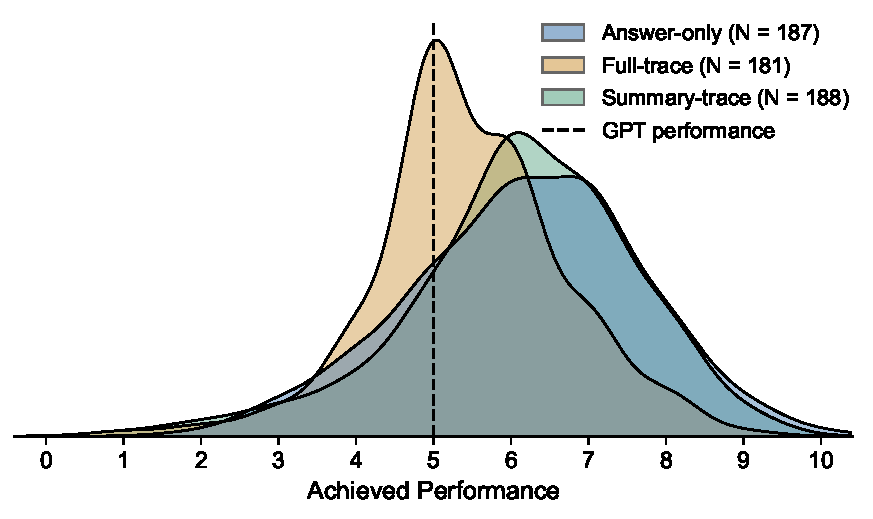
\includegraphics[width=0.8\linewidth]{comparison_3modes.pdf}
    \caption{Achieved performance (0-10) across trace formats. \textit{Answer-only} condition, $N=187$ (blue curve); \textit{Full-trace} condition, $N=181$ (orange curve); \textit{Summary-trace} condition, $N=188$ (green curve). The performance of the models is represented by a dashed vertical line 
    (both GPT-5 and gpt-oss-20b achieved a score of 5 on the set of 10 LSAT questions).}
    \label{fig:performance_comparison}
\end{figure}

    

\subsubsection{Overestimation Bias}
Perceived performance substantially exceeded actual performance in all conditions. In \textit{Answer-only} condition, participants estimated 7.92 items correct ($SD = 1.59$), while achieving 6.18 ($SD = 1.46$) correct items, yielding a significant overestimation, $t(186) = 11.63$, $p < .001$, $d = .85$. In \textit{Full-trace} condition, participants estimated 7.89 items correct ($SD = 1.71$), while achieving 5.46 correct items ($SD = 1.20$), also showing significant overestimation, $t(180) = 16.13$, $p < .001$, $d = 1.20$. In \textit{Summary-trace} condition, participants estimated 8.07 items correct ($SD = 1.56$), while achieving 6.13 ($SD = 1.44$) correct items, again showing significant overestimation, $t(187) = 13.21$, $p < .001$, $d = .96$.


Perceived performance did not differ significantly across conditions, $F(2, 553) = 0.66$, $p = .520$, $\eta^2 = .002$. However, the magnitude of overestimation differed significantly by condition, $F(2, 553) = 5.60$, $p = .004$, $\eta^2 = .020$. Participants in \textit{Full-trace} condition showed the largest overestimation bias ($M = 2.43$, $SD = 2.02$), followed by \textit{Summary-trace} ($M = 1.94$, $SD = 2.01$) and \textit{Answer-only} ($M = 1.74$, $SD = 2.04$). Tukey-adjusted post-hoc comparisons showed that overestimation was significantly larger in \textit{Full-trace} condition than in \textit{Answer-only} ($M_{\mathrm{diff}} = 0.69$, $p_{\mathrm{adj}} = .003$). \textit{Summary-trace} did not differ significantly from \textit{Answer-only} ($M_{\mathrm{diff}} = 0.20$, $p_{\mathrm{adj}} = .610$) or \textit{Full-trace} ($M_{\mathrm{diff}} = -0.49$, $p_{\mathrm{adj}} = .054$). The preregistered ordering (H1: greatest metacognitive accuracy under \textit{Summary-trace}, least under \textit{Answer-only}) was not confirmed).s


\begin{figure}[!htp]
    \centering
    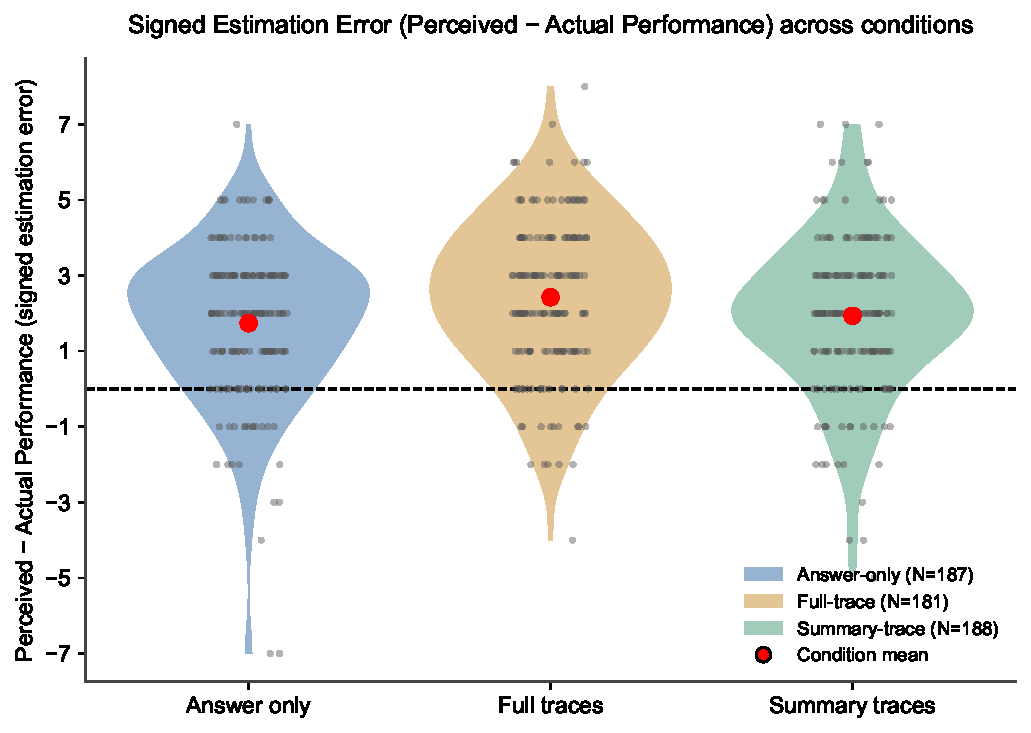
\includegraphics[width=0.7\linewidth]{violin_estimation_error.pdf}
    \caption{Performance estimation bias (perceived-actual performance) across conditions. Positive values indicate overestimation.}
    \label{fig:violin_plot}
\end{figure}

Together, these results indicate that participants across all conditions overestimated their performance, but this miscalibration was most pronounced in the full reasoning trace condition. Notably, \textit{Full-trace} participants performed worst objectively while perceiving their performance as comparable to participants in the other conditions, resulting in the largest overestimation gap. Summary traces did not significantly worsen miscalibration relative to the answer-only baseline, although participants' self-beliefs remained inflated.


\begin{table}[!htp]
\centering
\caption{ANOVAs with descriptives by condition. Values are means with standard deviations in parentheses.}

\begin{tabular}{lcccccccc}
\hline
DV                    & \textit{Answer-only}             & \textit{Full-trace}                 & \textit{Summary-trace} & F & df1 & df2 & p & \multicolumn{1}{l}{$\eta^2$} \\ \hline
Achieved  &    6.18 (1.46)      &      5.46 (1.20)     &      6.13 (1.44)           &       15.65           &              2        &      553                &      <.001***           &            .054         \\
Perceived &    7.92 (1.59)      &      7.89 (1.71)     &      8.07 (1.56)          &       0.66       &             2           &       553             &        .520       &           .002       \\
Overestimation &    1.74 (2.04)      &        2.43 (2.02)    &        1.94 (2.01)          &     5.60             &             2         &     553                &      .004**            &           .020           \\
NASA-TLX     & 43.85 (13.09)  & 45.06 (14.26)  & 45.42(13.36)  &  .688 & 2 & 553 & .503 & .002  \\
TSQ                     & 3.61 (0.76)  & 3.81 (0.72)  & 3.83 (0.72)  & 4.94  & 2 & 553 & .007** & .018  \\                UEQ-S                     & 1.18 (1.08)  & 1.59 (1.02)  & 1.54 (0.99)  & 8.58  & 2 & 553 & <.001*** & .030  \\
SUS                     & 78.48 (15.34)  & 76.01 (19.32)  &  77.87 (17.00) & 1.016 & 2 & 553 & .363 & .004  \\


\hline
\end{tabular}

%\raggedright \small  \textit{Note 1}. Achieved corresponds to achieved performance. Perceived corresponds to the perceived performance (self-estimation). Overestimation corresponds to the difference between perceived and achieved performance. 

%\small  \textit{Note 2}. Reported are one-way between-subjects ANOVAs with condition (baseline, full trace, summary trace) as the factor. $\eta^2$ denotes effect size. Significance levels: *$p < .05$, **$p < .01$, ***$p < .001$.

%\small \textit{Note 3}. NASA-TLX scale from 0-100

%\small  \textit{Note 4}. SUS scale from 0-100

%\small \textit{Note 5}. UEQ-S scale from -3 to 3 as stated in \ref{add ueq-s paper here}

\raggedright \small \textit{Note}. Reported are descriptive statistics and one-way between-subjects ANOVAs with condition as the factor. The $p$ column refers to the omnibus ANOVA test, not pairwise comparisons. Pairwise condition differences were examined using Tukey-adjusted post-hoc comparisons and are reported in the text where relevant. Achieved performance, perceived performance, and overestimation are reported as number of items out of 10. Overestimation corresponds to perceived minus achieved performance. NASA-TLX and SUS are reported on 0--100 scales. TSQ is reported on a 1--5 scale. UEQ-S is reported on a $-3$ to $+3$ scale, where higher values indicate a more positive user experience. $\eta^2$ denotes effect size. Significance levels: *$p < .05$, **$p < .01$, ***$p < .001$.
\end{table}

\subsection{Metacognitive Sensitivity}


To examine whether participants' self-assessments were related to their actual performance, we computed within-condition correlations between perceived and achieved performance. In all three conditions, correlations were low and non-significant: \textit{Answer-only}, $r(185) \approx .10$, $p = .166$; \textit{Full-trace}, $r(179) \approx .07$, $p = .344$; \textit{Summary-trace}, $r(186) \approx .10$, $p = .168$. This indicates that participants' performance estimates were weakly related to their actual scores, regardless of trace format. In other words, we found no evidence that any condition helped participants form more accurate self-assessments after completing all the tasks, as the format of reasoning traces did not improve the alignment between perceived and achieved performance. 

To test whether participants discriminated correct from incorrect responses within each condition, we ran paired-samples $t$-tests comparing $\overline{c_{+}}$ and
$\overline{c_{-}}$. The effect was significant in every condition: \textit{Answer-only}, $t(185) = 6.27$, $p < .001$, $d_z = 0.46$, $M_{\Delta} = 0.065$; \textit{Full-trace}, $t(180) = 4.99$, $p < .001$, $d_z = 0.37$, $M_{\Delta} = 0.048$; \textit{Summary-trace}, $t(187) = 5.57$,
$p < .001$, $d_z = 0.41$, $M_{\Delta} = 0.062$. Across conditions, however, the size of the gap did not differ (\textit{Answer-only}: $M = 0.065$, $SD = 0.141$; \textit{Full-trace}: $M = 0.048$, $SD = 0.129$; \textit{Summary-trace}: $M = 0.062$, $SD = 0.152$), $F(2, 552) = 0.78$, $p = .461$, $\eta^2 = .003$.%





To assess whether AI exposure changed how well participants' confidence ratings tracked their actual performance at trial-level, we computed four trial-level metacognitive indices from the ten LSAT items per participant. Correctness was coded as $1/0$, and the 0--100 confidence slider was rescaled to $[0,1]$. Table~\ref{tab:meta-indices} reports the descriptives and ANOVA summaries for all four indices of metacognitive sensitivity (for an introduction, see \citet{rahnev2025comprehensive}). We employed (AUC, Brier Score, calibration and discrimination\footnote{For AUC and discrimination one participant had to be removed due to scoring 10/10.}) \footnote{We do not report meta-d' or M-ratio as reliable estimation, even under the HMeta-d hierarchical Bayesian estimator, requires substantially more trials per participant than our 10-item battery.}. 
As a first intuitive sensitivity index, we computed each participant's
\emph{confidence gap}, $\Delta_{\text{disc}} = \overline{c_{+}} - \overline{c_{-}}$, defined as the difference between mean confidence on correct trials ($\overline{c_{+}}$) and mean confidence on incorrect trials ($\overline{c_{-}}$). Positive values indicate that confidence was higher when the response was right than when it was wrong; values near zero indicate insensitivity. %To test whether participants discriminated correct from incorrect responses within each condition, we ran paired-samples $t$-tests comparing $\overline{c_{+}}$ and $\overline{c_{-}}$. The effect was significant in every condition: \textit{Answer-only}, $t(185) = 6.27$, $p < .001$, $d_z = 0.46$, $M_{\Delta} = 0.065$; \textit{Full-trace}, $t(182) = 4.98$, $p < .001$, $d_z = 0.37$, $M_{\Delta} = 0.047$; \textit{Summary-trace}, $t(188) = 5.61$, $p < .001$, $d_z = 0.41$, $M_{\Delta} = 0.062$. 

\begin{table}[H]
\centering
\caption{One-way ANOVAs with descriptives by condition for the four
metacognitive indices. Values are means with standard deviations in
parentheses; all indices are computed at the individual level (one
value per participant) on a $[0,1]$ scale.}
\label{tab:meta-indices}
\resizebox{\linewidth}{!}{%
\begin{tabular}{lccccllll}
\hline DV                                & Answer-only M(SD)  & Full-trace M(SD)      & Summary-trace M(SD)   & F     & df1 & df2 & $p$       & $\eta^2$ \\ \hline
Discrimination ($\Delta_{\text{disc}}$)  & 0.065 (0.141)   & 0.048 (0.129)   & 0.062 (0.152)   & 0.78  & 2   & 552 & .461      & .003 \\
AUROC2                                   & 0.586 (0.206)   & 0.562 (0.192)   & 0.586 (0.202)   & 0.87  & 2   & 552 & .418      & .003 \\
Calibration bias                         & 0.189 (0.179)   & 0.263 (0.183)   & 0.221 (0.179)   & 7.83  & 2   & 553 & $<$.001***& .028 \\
Brier score                              & 0.289 (0.111)   & 0.341 (0.116)   & 0.296 (0.111)   & 11.58 & 2   & 553 & $<$.001***& .040 \\
\hline
\end{tabular}}
\end{table}


As a second, distribution-free sensitivity index we computed the non-parametric Type-2 ROC area, defined as the probability that a randomly drawn correct trial received a higher confidence rating than a randomly drawn incorrect trial, with ties contributing $0.5$. AUROC2 is bounded in $[0,1]$, equals $0.5$ at chance, and unlike
$\Delta_{\text{disc}}$ depends only on the rank-order of confidence which makes it robust to wicked distributions. Mean AUROC2 was nearly identical across conditions
(baseline: $M = 0.586$, $SD = 0.206$; full: $M = 0.562$, $SD = 0.192$;
summary: $M = 0.586$, $SD = 0.202$) and conditions did not differ, $F(2, 552) = 0.87$, $p = .418$, $\eta^2 = .003$.

Whereas the two indices above quantify \emph{sensitivity} (whether confidence \emph{discriminates} correct from incorrect trials), we
next examined \emph{calibration} (whether confidence \emph{matches} accuracy in absolute terms). For each participant, we computed
$\mathrm{calibration} = \overline{c} - \mathrm{accuracy}$, where $\overline{c}$ is mean confidence and $\mathrm{accuracy}$ is the proportion of items answered correctly. Positive values indicate overconfidence, negative values indicate underconfidence. Calibration differed between conditions, $F(2, 553) = 7.83$, $p < .001$, $\eta^2 = .028$.
All conditions were overconfident on average, but the \textit{Full-trace} condition ($M = 0.263$, $SD = 0.183$) showed greater overconfidence
than baseline ($M = 0.189$, $SD = 0.179$; Tukey HSD, $p < .001$); the \textit{Summary-trace} condition ($M = 0.221$, $SD = 0.179$) fell between the
two and did not differ reliably from either (vs. \textit{Answer-only}, $p = .19$; vs. \textit{Full-trace}, $p = .068$).


As an integrated measure that combines calibration and resolution, we computed the Brier score, $\mathrm{BS} = \tfrac{1}{n}\sum_{i}(c_i - y_i)^2$, i.e.\ the mean squared error of confidence treated as a probabilistic forecast of correctness $y_i \in \{0,1\}$. It rewards forecasts that are both well-calibrated and discriminating, and lower values indicate forecasts that are simultaneously well-calibrated and informative; a participant who reports a confidence of 50 on every trial attains a Brier score of $0.25$. Conditions differed reliably, $F(2, 553) = 11.58$, $p < .001$, $\eta^2 = .040$. The \textit{Full-trace} condition produced the worst (highest) Brier scores ($M = 0.341$, $SD = 0.116$) and was reliably worse than both \textit{Answer-only} ($M = 0.289$, $SD = 0.111$; Tukey HSD, $p < .001$) and \textit{Summary-trace} ($M = 0.296$, $SD = 0.111$; $p < .001$); \textit{Answer-only} and \textit{Summary-trace} did not differ ($p = .80$). Together, these results indicate that participants' metacognitive sensitivity was relatively weakened in the \textit{Full-trace} condition.



\subsubsection{Collaborative AI Metacognition Scale (CAIMS)}
We use CAIMS as a self-report index of users' disposition to engage metacognitively with AI.
Metacognitive engagement during AI-assisted reasoning was assessed using the Collaborative AI Metacognition Scale \cite{Sidra03042026}, which measures Planning, Monitoring, and Evaluation of one's thinking while working with AI (all items rated on a 1--5 scale; higher scores indicating a disposition for greater metacognitive engagement in AI Interaction).

Self-reported metacognitive collaboration on the CAIMS was high across the board and increased monotonically from \textit{Answer-only} through \textit{Full-trace} to \textit{Summary-trace} on every
subscale (Table~\ref{tab:caims-means}); the one-way ANOVA reached
significance only for evaluation, $F(2, 553) = 3.08$, $p = .047$,
$\eta^2 = .011$ (\textit{Summary-trace} $>$ \textit{Answer-only}, Tukey $p = .036$). The correlational picture, however, ran counter to what a genuine
metacognitive-monitoring account would predict: pooling across all 556 participants (Table~\ref{tab:caims-overall}), every CAIMS scale
predicted \emph{larger} signed overestimation bias and \emph{larger} absolute metacognitive error (all $r \approx .12$--$.18$,
$p \leq .005$, Holm-significant).

Extending the analysis to the trial-level indices of metacognitive sensitivity reinforces the pattern: CAIMS
positively predicted mean confidence (planning $r = .28$, monitoring $r = .27$, evaluation $r = .33$, total $r = .33$), trial-level calibration error (all $r \approx .26$-$.31$), and Brier scores (all $r \approx .22$-$.27$; all of these Holm-significant at
$p < .001$), and showed small \emph{negative} associations with the two rank-based sensitivity indices (confidence gap and AUROC2; planning, evaluation, and total Holm-significant for both indices, $r$'s between $-.14$ and $-.08$; monitoring not surviving correction). Self-reported metacognitive literacy, therefore, tracks the \emph{level} of inflated confidence and the calibration error it
produces while, if anything, being inversely related to the \emph{informativeness} of confidence.

Crucially, the effect is not specific to the trace conditions: in
\textit{Answer-only} evaluation still predicted absolute miscalibration, $r = .23$, $p = .002$,
Holm $p = .006$, so the correlation cannot be reduced to the manipulation. The signed bias correlations were nevertheless
strongest in the \textit{Summary-trace} condition (planning $r = .24$, monitoring $r = .27$, evaluation $r = .21$, total $r = .28$; all $p \leq .006$),
accompanied by a slight performance drop (planning $\rightarrow$ score $r = -.17$, $p = .021$), indicating that \textit{Summary-trace}-condition participants who reported more metacognitive interaction literacy in terms of planning skewed specifically toward overestimation. This largely replicates \citet{FERNANDES2026108779}.


\begin{table}[!htp]
\centering
\caption{Overall (condition-agnostic) Pearson correlations between
CAIMS subscales and the three outcome variables. Values are
$r$ with 95\,\% CI; $N = 556$. Stars denote uncorrected $p$-values
(* $<.05$, ** $<.01$, *** $<.001$); $\dagger$ marks effects that
do not survive Holm correction across the 16 tests within each
outcome.}
\label{tab:caims-overall}
\begin{tabular}{lccc}
\hline Subscale     & Score                                & Calibration bias ($\Delta$)             & Absolute accuracy ($|\Delta|$)        \\ \hline
Planning             & $-.09^{*\dagger}$ $[-0.17,\,-0.00]$  & $.15^{***}$ $[0.07,\,0.23]$            & $.12^{**}$ $[0.04,\,0.20]$            \\
Monitoring           & $-.07$ $[-0.16,\,0.01]$              & $.15^{***}$ $[0.07,\,0.23]$            & $.15^{***}$  $[0.07,\,0.23]$           \\
Evaluation           & $-.06$  $[-0.15,\,0.02]$              &  $.17^{***}$ $[0.08,\,0.25]$            &  $.17^{***}$ $[0.09,\,0.25]$           \\
Total                & $-.09^{*\dagger}$ $[-0.17,\,-0.00]$  & $.18^{***}$  $[0.10,\,0.26]$            & $.16^{***}$ $[0.08,\,0.24]$           \\
\hline
\end{tabular}
\end{table}

\begin{table}[!htp]
\centering
\caption{CAIMS subscale and total descriptives by condition. Values
are means with standard deviations in parentheses on the 1--5 metric;
$F$, $p$, and $\eta^2$ are from one-way ANOVAs comparing the three
conditions.}
\label{tab:caims-means}
\resizebox{\linewidth}{!}{%
\begin{tabular}{lccccrrrr}
\hline Subscale     & Overall M(SD) & \textit{Answer-only} M(SD) & \textit{Full-trace} M(SD)   & \textit{Summary-trace} M(SD) & $F$  & df1 & df2 & $p$ \\ \hline
Planning             & 4.01 (0.70)   & 3.95 (0.72)    & 4.00 (0.67)  & 4.09 (0.72)   &  1.84 & 2   & 553 &  .160   \\
Monitoring           & 4.04 (0.66)   & 3.97 (0.71)    &  4.05 (0.65)  &  4.09 (0.61)   &  1.58 & 2   & 553 &  .208   \\
Evaluation           & 4.22 (0.64)   & 4.14 (0.66)    & 4.22 (0.63)  & 4.30 (0.63)   &  3.08 & 2   & 553 &  .047*  \\
Total                & 4.08 (0.59)   & 4.01 (0.60)    & 4.08 (0.58)  & 4.15 (0.57)   &  2.63 & 2   & 553 &  .073   \\
\hline
\end{tabular}}
\end{table}


%CAIMS scores were uniformly high across all conditions (Overall: $C1:M=4.01,SD=0.60;C2:M=4.08,SD=0.58;C3:M=4.15,SD=0.57$). %One-way ANOVAs revealed no significant differences across conditions for Planning, Monitoring or Overall metacognition.% A significant effect emerged for Evaluation, $F(2,556)=3.02, p = .049, \eta^2 = .011$. Tukey-adjusted post-hoc comparisons showed that participants in the Summary condition reported slightly higher evaluative metacognition than those in the Baseline condition ($M_{\mathrm{diff}} = 0.16, p_{\mathrm{adj}} = .038$). No other pairwise comparisons reached significance. 
% Effect sizes were negligible across all subfactors ($\eta^2 \leq .011$), and the uniformly high scores suggest a potential ceiling effect, which may have limited sensitivity to condition-induced differences.

% \begin{table}[H]
% \centering
% \caption{CAIMS descriptives and ANOVAs by condition. Values are means with standard deviations in parentheses.}
% \begin{tabular}{lcccccccc}
% \hline
% Scale & C1 M(SD) & C2 M(SD) & C3 M(SD) & F & df1 & df2 & p & $\eta^2$ \\ \hline
% Planning   & 3.95 (0.72) & 4.00 (0.67) & 4.09 (0.72) & 1.94 & 2 & 556 & .145 & .007 \\
% Monitoring & 3.97 (0.71) & 4.04 (0.65) & 4.10 (0.61) & 1.65 & 2 & 556 & .193 & .006 \\
% Evaluation & 4.14 (0.66) & 4.22 (0.63) & 4.30 (0.63) & 3.02 & 2 & 556 & .049* & .011 \\
% Overall    & 4.01 (0.60) & 4.08 (0.58) & 4.15 (0.57) & 2.71 & 2 & 556 & .067 & .010 \\
% \hline
% \end{tabular}

% \raggedright \small \textit{Note.} Scores are reported on a 1--5 scale (1 = \textit{Never}, 5 = \textit{Always}). Reported are one-way between-subjects ANOVAs with condition as the factor. 
% $\eta^2$ denotes effect size. Significance levels: *$p < .05$, **$p < .01$, ***$p < .001$.
% \label{tab:caims}
% \end{table}



\subsection{Perceived Task Workload and Trust}


We next examined perceived workload using the NASA-TLX. Overall task load did not differ significantly across conditions (\textit{Answer-only}: $M=43.85,SD=13.09$; \textit{Full-trace}: $M=45.06,SD=14.26$; \textit{Summary-trace}: $M=45.42,SD=13.36$; $F(2, 553) = 0.69$, $p = .503$, $\eta^2 =.002$. This suggests that exposure to reasoning traces, whether \textit{Full-trace} or summarized, did not impose additional task load relative to receiving only a final answer. The preregistered prediction (H2: highest load under \textit{Full-trace}) was accordingly not supported; the planned one-sided comparison of \textit{Full-trace} against \textit{Answer-only}, was not significant ($t(553) = 0.86$, $p = .196$; see Table~\ref{tab:prereg_verdicts}). Descriptive statistics for the overall NASA-TLX score and its six subscales are shown in Table~\ref{tab:nasa}.


Trust in the AI differed significantly across conditions $(F(2,553) = 4.94, p = .007,\eta^2 = .018)$. In all three conditions, trust ratings were significantly above the scale midpoint ($\mu = 3$): \textit{Answer-only} ($M = 3.61, SD = 0.76; t(186) = 10.91, p < .001, d = 0.80$), \textit{Full-trace} ($M = 3.81, SD = 0.72; t(180) = 15.08, p < .001, d = 1.12$), and \textit{Summary-trace} ($M = 3.83, SD = 0.72; t(187) = 15.64, p < .001, d = 1.14$). 
The preregistered ordering (H3: \textit{Full-trace} $\geq$ \textit{Summary-trace} $>$ \textit{Answer-only}) was confirmed for trust (see Table~\ref{tab:prereg_verdicts}).  Participants in the \textit{Answer-only } condition reported significantly lower trust than those in both the \textit{Full-trace} condition (\textit{Summary-trace}: $t(553) = 2.84$, $p = .002$; \textit{Full-trace}: $t(553) = 2.57$, $p = .005$; one-sided), the linear trend across the predicted order was significant ($d = 0.27$, $p = .005$), and a distribution-free Jonckheere--Terpstra test agreed ($p = .003$). 
No significant difference was found between the \textit{Full-trace} and \textit{Summary-trace} conditions r ($t(553) = 0.24$, $p = .810$).

%Tukey-adjusted post-hoc comparisons revealed that participants in the \textit{Answer-only }condition reported significantly lower trust than those in both the \textit{Full-trace} condition ($p_{adj} = \new{.028}$) and the \textit{Summary-trace} condition ($p_{adj} = \new{.013}$). No significant difference was found between the \textit{Full-trace} and \textit{Summary-trace} conditions ($p_{adj} = \new{.969}$).


\subsubsection{Follow-Up Ratings}
After each problem, participants rated their confidence in their own answer on a 0--100 slider. This trial-level confidence measure differs from the global performance estimate reported after task completion (used to compute overestimation above, see section \ref{sec:achieved_performance}) and in Conditions \textit{Full-trace} and \textit{Summary-trace}, they additionally rated the perceived usefulness of the reasoning traces, whether the reasoning matched the model's final answer, and their confidence in the model's answer. Confidence in one's own answer did not differ significantly across conditions ($F(2,553) = 2.47, p = .085, \eta^2 = .009$). 
The preregistered ordering for confidence (H3), however, was not verified. \textit{Full-trace} did not exceed \textit{Answer-only} ($t(553) = 0.17$, $p = .864$), contradicting the predictied order. Yet, the preregistered comparison of \textit{Summary-trace} against \textit{Answer-only}  was significant ($t(553) = 2.01$, $p = .045$), and a significant quadratic contrast ($p = .027$) shows that confidence was the highest in the \textit{Summary-trace} condition and did not increase with the amount of reasoning shown (see Table~\ref{tab:prereg_verdicts}).
Among conditions exposed to reasoning traces, participants did not differ significantly in perceived usefulness of the reasoning ($F(1,367) = 2.53, p = .112, \eta^2 = .007$) or confidence in the model's answer ($F(1,367) = 0.42, p = .518, \eta^2= .002$). However, participants in the full-trace condition rated the reasoning as matching the model's final answer more closely than those in the \textit{Summary-trace} condition $(F(1,367) = 4.15, p = .042, \eta^2= .011$; \textit{Full-trace}: $M = 80.43, SD = 14.41; \textit{Summary-trace}: M = 76.88, SD = 18.69)$. This suggests that while full traces were perceived as more internally coherent, this did not translate into higher usefulness ratings or greater confidence in the model, which is consistent with \cite{von2025knowing}.


\begin{table}[!htp]
\centering

\caption{ANOVAs with descriptives by condition for follow-up questions after each task. Values are means with standard deviations in parentheses.}

\begin{tabular}{lccccllll}
\hline DV             & \textit{Answer-only} & \textit{Full-trace}       & \textit{Summary-trace}    & F    & df1 & df2 & $p$     & $\eta^2$ \\ \hline
Confidence (own answer)   & 80.68 (12.39)  & 80.92 (14.98)  & 83.43 (12.29)  & 2.47 & 2  & 553 & .085  & .009     \\
Usefulness of reasoning   & --  & 78.06 (15.91)   & 75.17 (18.77)   & 2.53 & 1   & 367  & .112     &  .007  \\
Reasoning matched answer  & --  & 80.43 (14.41)  & 76.88 (18.69)  & 4.15 & 1   & 367  & .042*   & .011   \\
Confidence in model answer    & --   & 77.64 (16.15)   & 76.53 (16.92)   & .42 & 1   & 367  &  .518 & .001      \\
\hline
\end{tabular}

\raggedright \small  \textit{Note}: Reported are one-way ANOVAs with condition as the factor. For Confidence (in own answer), all three conditions (\textit{Answer-only}, \textit{Full-trace}, \textit{Summary-trace}) were included. For the other follow-ups, only \textit{Full-trace} vs. \textit{Summary-trace} conditions were compared (\textit{Answer-only }did not include these questions). Means are on a 0--100 scale. $\eta^2$ denotes effect size. Significance levels: *$p < .05$, **$p < .01$, ***$p < .001$.
\end{table}


\subsection{System Usability}
\subsubsection{System Usability Scale} System usability was measured using the SUS-S questionnaire \cite{brooke1996sus,bangor2008empirical}, did not differ significantly across conditions, $F(2, 553) = 1.02$, $p = .363$, $\eta^2 = .004$. Mean SUS scores were high across all conditions: \textit{Answer-only} ($M = 78.48$, $SD = 15.34$), \textit{Full-trace} ($M = 76.01$, $SD = 19.32$), and \textit{Summary-trace} ($M = 77.87$, $SD = 17.00$). Tukey-adjusted post-hoc comparisons showed no significant pairwise differences between conditions, all $p_{\mathrm{adj}} \geq .357$. The preregistered ordering (H5: \textit{Answer-only} $\geq$ \textit{Summary-trace} $>$ \textit{Full-trace}) was not supported. The observed means followed the predicted order ($76.01 < 77.87 < 78.48$), but neither planned comparison reached significance (one-sided $p \geq .086$; linear trend $d = 0.14$; Table~\ref{tab:prereg_verdicts}).

\subsubsection{User Experience}
We next examined participants' subjective user experience using the UEQ-S \cite{alberola2018creation}\footnote{Our implementation presented UEQ-S item 4 as \textit{Clear} $\ldots$ \textit{Confusing}, whereas the published instrument places the negative term on the left for all eight items (\textit{confusing} $\ldots$ \textit{clear}). We therefore reverse-scored this item before the $-3$ to $+3$ recode, as the scoring convention requires.}. The UEQ-S provides separate scores for Pragmatic Quality, reflecting task-oriented qualities such as clarity, efficiency, and ease of use, and Hedonic Quality, reflecting qualities such as interest, excitement, and novelty. Scores range from $-3$ to $+3$, with higher values indicating a more positive user experience. Descriptive statistics are reported in Table~\ref{tab:ueqs}.

\begin{table}[!htp]
\centering
\caption{(UEQ-S) Pragmatic, Hedonic and Overall scales per condition for the UEQ-s questionnaire, M(SD)}
\begin{tabular}{lcccccccc}
\hline
                  & \textit{Answer-only}    & \textit{Full-trace}   & \textit{Summary-trace}   & F & df1 & df2 & $p$     & $\eta^2$ \\ \hline
Pragmatic Quality & 1.63 (1.07) & 1.86 (1.11) & 1.77 (1.03) & 2.24 & 2 & 553 & .108 & .008 \\
Hedonic Quality   & 0.73 (1.39) & 1.31 (1.16) & 1.31 (1.21) & 13.08 & 2 & 553 & <.001*** & .045 \\
UEQ-S Overall     & 1.18 (1.08) & 1.59 (1.02) & 1.54 (0.99) & 8.58 & 2 & 553 & <.001*** & .030 \\  
\hline
\end{tabular}

\raggedright \small \textit{Note}: Reported are one-way ANOVAs with condition as the factor. All three conditions (\textit{Answer-only}, full reasoning, summary reasoning) were included. Means and Standard Deviations are reported on the UEQ-S scale, ranging from $-3$ to $+3$, where higher values indicate a more positive user experience. $\eta^2$ denotes effect size.  Significance levels: *$p < .05$, **$p < .01$, ***$p < .001$.
\label{tab:ueqs}
\end{table}


Condition had a significant effect on two of the three UEQ-S measures. Pragmatic Quality did not differ across conditions, and no pairwise contrast approached significance (\textit{Full-trace} \textit{vs}. \textit{Answer-only}, $p_{adj} = .092$; \textit{Summary-trace} \textit{vs}. \textit{Answer-only}, $p_{adj} = .406$; \textit{Full-trace} \textit{vs}. \textit{Summary-trace}, $p_{adj} = .687$). For Hedonic Quality, both \textit{Full-trace} and \textit{Summary-trace} were rated significantly higher than \textit{Answer-only} (both $p_{adj} < .001$), with no significant difference between \textit{Full-trace} and \textit{Summary-trace} ($p_{adj} = .997$). The same pattern was observed for the UEQ-S overall measurement. Both \textit{Full-trace} ($p_{adj} < .001$) and \textit{Summary-trace} ($p_{adj} = .001$) were rated significantly higher than \textit{Answer-only}, while \textit{Full-trace} and \textit{Summary-trace} did not differ significantly ($p_{adj} = .646$).
Thus, reasoning traces improved subjective user experience relative to the \textit{Answer-only}, and did so entirely through the hedonic half of the scale. However, full and summary traces were experienced similarly overall, suggesting that the more verbose full traces did not provide an additional subjective experience benefit over summarized traces.

\subsection{Mechanism: Does the trace-induced trust gain explain miscalibration?}
\label{sec:mediation}
The metacognitive sensitivity analyses above show that trace exposure, particularly exposure to full reasoning traces, inflates participants' confidence in their own performance, but they leave the mechanism underspecified.
One possibility is that the trace-rich interaction shifts participants' subjective appraisal of the AI (perceived trustworthiness, perceived engagement), and that they then use this appraisal as evidence of their joint competence. Because we collected both TSQ trust ratings and UEQ hedonic appeal in the same session, this account is testable within the present sample.
To probe the mechanism behind the condition effect, we fit a parallel multiple-mediator model in \texttt{lavaan} with condition as a three-level dummy-coded predictor (\textit{Answer-only} reference), trust (TSQoverall), and UEQ hedonic as parallel mediators, and overestimation bias ($\Delta = \mathrm{Estimate} - \mathrm{Score}$) as the outcome; all variables were $z$-standardized and indirect effects were tested with $5{,}000$ percentile bootstrap samples ($N = 556$).

Both trace conditions raised trust ($a_{1,\text{full}} = 0.27$, $p = .010$; $a_{1,\text{summary}} = 0.29$, $p = .005$) and hedonic appeal ($a_{2,\text{full}} = 0.45$; $a_{2,\text{summary}} = 0.45$; both $p < .001$), but only hedonic appeal predicted overestimation once trust was partialled out ($b_{2} = 0.15$, $p = .009$; $b_{1} = 0.09$, $p = .13$), so the indirect path through hedonic was significant for both conditions (\textit{Full-trace}: $\hat{\beta} = 0.066$, 95\,\% CI $[0.016, 0.130]$; \textit{Summary-trace}: $0.065$, $[0.016, 0.129]$) whereas the trust path was not. Single-mediator sensitivity models showed that trust \emph{does} carry an indirect effect on its own (\textit{Full-trace}: $0.048$, $[0.008, 0.099]$), but this effect is absorbed by hedonic when both are entered jointly: trust and hedonic correlate $r = .65$ ($R^{2} = .42$, tolerance $= .58$, VIF $= 1.72$ for trust and $1.77$ for hedonic in the $b$-path), so when entered together the trust slope shrinks by $51\%$ (solo $b = 0.18 \to$ joint $b = 0.09$) while the hedonic slope shrinks by only $28\%$ ($0.20 \to 0.15$). The two mediators jointly explained variance in overestimation over and above condition, $F(2, 551) = 12.90$, $p < .001$, but this shared variance is captured almost entirely by hedonic appeal, indicating that UEQ hedonic provides a more comprehensive proxy for the relevant subjective appraisal. The \textit{Full-trace} condition retained a direct effect ($c'_{f} = 0.25$, $p = .018$; partial mediation), while the \textit{Summary-trace} condition was fully mediated ($c'_{s} = 0.01$, $p = .95$).

The AI interaction inflates participants' subjective appraisal of the exchange, which they then use as evidence of their own performance. Once the variance shared by trust and hedonic is partitioned, only the unique-to-hedonic variance predicts overestimation, suggesting the active ingredient is closer to a fluency/affect signal than to calibrated trust, consistent with processing-fluency accounts of metacognitive misattribution \cite{alter2009uniting}.


\subsection{Qualitative Analysis}


%In this section, we present the results of the qualitative analysis. We analyzed the qualitative data collected during the study using an inductive thematic approach \cite{clarke2017thematic}. This included the responses to an open-ended question at the end of the questionnaire and their comments on the model reasoning and answer. The analysis provided insight into how participants interacted with the AI chatbot and their perceptions of it, where recurrent themes were found (see \autoref{sec:qualitative_C2} and \autoref{tab:qualitative_C3}).

To understand how participants engaged with reasoning traces (\textit{Full-trace} and \textit{Summary-trace} conditions), we conducted an inductive thematic analysis \cite{clarke2017thematic} of participants' open-ended responses to ``\textit{Please describe how you used the AI Chatbot}'' and ``\textit{Please share any comments about the reasoning or the answer}''. Across both conditions, four recurring interaction patterns emerged: cognitive offloading, guided reasoning, calibrated comparison, and trace burden. We report the frequency of each pattern and use representative quotes to interpret the quantitative findings\footnote{ C2 and C3 prefixes on participant IDs correspond to the \textit{Full-trace} and \textit{Summary-trace} conditions, respectively.}.



\subsubsection{Full-trace Condition}

%In Condition 2, participants were exposed to full reasoning traces and could reveal the model’s final answer. To examine how participants used the model in this condition, we conducted a qualitative analysis of their responses to the open-ended question "A qualitative analysis of the open-ended question "Please describe how you used the AI Chatbot", revealing different perceptions of the AI and highlighting distinct modes of interaction.
In the \textit{Full-trace} condition, participants saw the model's reasoning trace before it revealed its final answer. Participants' descriptions referred almost exclusively to the reasoning content, and the reveal-answer button itself was rarely mentioned. We therefore interpret the patterns as responses to the traces.

%Participants were grouped into six categories. Participants' descriptions primarily referred to the model’s reasoning and explanations, where the reveal-answer button itself was not salient. Therefore, the qualitative findings are interpreted mainly as responses to the presence of full reasoning traces. 

Four main patterns emerged (Table~\ref{tab:qualitative_C2}).
The largest group (Group 1, $35.9\%$) used the model as primary source of answers, asking it for answers or following its suggestions with limited independent evaluation. For example, participant C2-P122 wrote that the chatbot was ``\textit{spot on}'' and that they ``\textit{just followed exactly what it suggested}''. Similarly, C2-P130 described pasting the question and answer options and having the model ``\textit{choose the best answer}''. This pattern suggests that full traces led to delegation rather than support evaluation and functioning as a transparency mechanism. Instead, the reasoning seemed to act like the placebic explanations described by \citet{eiband2019impact}, where the presence of fluent justifications increased trust independently of whether participants engaged with its content. This interpretation is consistent with participants' trust ratings in the \textit{Full-trace} condition despite its lower task accuracy.

%The largest group of participants used the AI as a primary answer source or engaged in cognitive offloading, asking the model for answers or following its suggested response with limited evidence of independent evaluation (Group 1: $65/183, 35.3\%$). These participants described asking the model for answers, following the generated response, or using the model output as the basis for their own answer. For example, C2-P122 wrote that the chatbot was ``\textit{spot on}'' and that they ``\textit{just followed exactly what it suggested}.'' Similarly, C2-P130 described pasting in the question and answer options and having the model ``\textit{choose the best answer}.'' This pattern suggests that full reasoning traces may increase the perceived understanding of the model. However, this trust was not always calibrated. In some cases, the reasoning trace appeared to support cognitive offloading rather than independent evaluation.

A second large group (Group 2, $57/181, 31.5\%$) used the trace as a guided reasoning aid, asking follow-up questions, using the model to break down problems, or relying on the trace to choose among options. Participant C2-P22 wrote that the model ``\textit{guided me step by step},'' and ``\textit{increased my confidence in selecting the right answer}.''
This pattern is the qualitative counterpart to the illusion of understanding documented by \citet{fisher2021harder}, where fluent, well-organized reasoning traces gave participants a sense that they had grasped the problem, even when their task performance did not improve. The same mechanism may explain the largest overestimation observed in the \textit{Full-trace} condition, where participants felt they had reasoned through the problem, when in practice, they simply trusted the model reasoning.

%C2-P70 similarly reported asking follow-up questions ``\textit{to understand its reasoning}.''  
%This pattern suggests that full reasoning traces can make the model more inspectable and useful for reasoning support, which may lead to a higher confidence in the model's answer, therefore leading to a higher overestimation (C2 was the condition with the highest overestimation level).


A third smaller group ($37/181, 20.4\%$) used the model for calibrated comparison. Participants first formed their own answer, then used the model's reasoning to confirm or challenge it. C2-P34 reported that while the AI was reasoning, they ``reasoned through the problem myself,'' and then checked the model’s logic against their own. %Similarly, C2-P41 described trying to solve the questions independently and using the chatbot to ``\textit{double check.}'' This pattern suggests that full reasoning traces can support calibrated trust.
This pattern constitutes genuine human–AI synergy \cite{vaccaro2024combinations} in which the user retains the cognitive work and uses the trace as a point of comparison rather than a replacement for their own reasoning.


Finally, a notable subset (Group 4, $18/181, 9.9\%$) experienced the trace as a burden, being too long, confusing, or something they actively shortened. C2-P53 wrote that the responses were ``\textit{so incredibly long}'' that reading them thoroughly would take too much time. Participant C2-P138 reported asking the model to ``\textit{dumb it down}'' and ``\textit{summarize it to be shorter}'' when the reasoning was confusing. These comments highlight the problem in XAI literature that the same verbosity that promises transparency can become an obstacle, with several participants reproducing the \textit{Summary-trace} condition on their own initiative.

%A notable subset of participants experienced the full reasoning traces as burdensome or difficult to manage (Group 4: $19/183, 10.4\%$). Participants in this group described explanations as too long, confusing, overwhelming, or something they skimmed or asked the model to shorten. C2-P53 wrote that the responses were ``\textit{so incredibly long}'' that reading them thoroughly would take too much time, while C2-P138 reported asking the model to ``\textit{dumb it down}'' and ``\textit{summarize it to be shorter}'' when the reasoning was confusing. Similarly, C2-P25 reported asking the chatbot to answer with ``\textit{short reasoning responses as to not get overwhelmed with too much information}''. C2-P71 described skimming the reasoning when the model’s answer matched theirs and reading more carefully when it differed. These comments indicate a transparency–burden tradeoff: full reasoning traces gave participants more information to review, but it also increased reading and time spent on task. \daniela{link with too fluent explanations}

%Overall, the C2 qualitative data suggest that full reasoning traces had mixed effects. They made the model more transparent and useful for some participants, supporting guided reasoning and calibrated comparison. At the same time, they also encouraged answer delegation for a larger subset of participants and created cognitive-load and usability costs for others. 


\subsubsection{Summary-trace Condition}
In the \textit{Summary-trace} condition, participants saw a short summary of the model's reasoning together with its final answer. When analyzing the qualitative data, three patterns accounted for 95\% of responses (Table~\ref{tab:qualitative_C3}).


The largest group (38.8\%) used the traces as a reasoning and decision-support aid. These participants described reading the summarized reasoning, using it to evaluate options, or asking follow-up questions. C3-P64 wrote that the chatbot ``\textit{helped break down each question}'' and clarified relationships between statements and assumptions. The summary appeared to provide enough rationale to support reasoning without imposing the costs of a full trace, consistent with the \textit{Full-trace} burden pattern.

%The largest group used the AI as a summary-based reasoning and decision-support tool ($74/189, 39.2\%$). These participants described reading the model's summarized reasoning, using it to evaluate answer options, asking follow-up questions, or using the explanation to reach a conclusion. For example, C3-P2 reported they used the model ``\textit{mostly for its reasoning}'' and that the reasoning was more important than the final answer. C3-P23 similarly reported reading the model's reasoning, evaluating its suggested answer, and then selecting the best choice. Other participants described the summary as helping them work through difficult reasoning problems: C3-P64 wrote that the chatbot ``\textit{helped break down each question}'' and clarified relationships between statements and assumptions. These responses suggest that the summary trace often provided enough rationale for participants to use the model as a reasoning aid without requiring them to process a full trace.

A second group (28.7\%) used the summary for calibrated comparison. These participants first formed their own answer, then compared it to the model's. C3-P58 provides a particularly clear example: ``\textit{(...)When I disagreed with the model, I checked its reasoning against my own. If I was not persuaded then I would stick with my answer}''. The proportion of calibrated comparison users was similar across the \textit{Full-trace} and \textit{Summary-trace} conditions (20.4\% vs. 28.7\%), suggesting that whether participants adopt this stance reflects the user as much as the interface.

%A second group used the AI for independent verification or calibrated comparison ($54/189, 28.6\%$). These participants first formed their own answer, intuition, or reasoning, and then compared it with the model's summary and final answer. C3-P1 wrote that they chose their own answer while the model responded and, when the answers did not match, read the reasoning to determine which was right. C3-P53 similarly described first forming their own reasoning and then comparing the model's reasoning with theirs before reaching a final conclusion. C3-P58 provides a particularly clear example of calibrated use: `` \textit{(...) When I disagreed with the model, I checked its reasoning against my own. If I was not persuaded then I would stick with my answer.}'' 
%This pattern suggests that the summary of reasoning traces supported participants' metacognitive accuracy, as they were not simply accepting the model's answer but rather using the summary as a compact comparison point for their own reasoning.

A third group (27.7\%) used the model as their primary source of answers, copying questions into it and selecting the answer based on its output with limited independent evaluation. C3-P127 stated, ``\textit{On most answers I solely relied on the AI Chatbot. I copy/pasted the question and answers and allowed it to give me the answer},'' Notably, this offloading rate was lower in the \textit{Summary-trace} condition than in \textit{Full-trace} (27.7\% vs. 35.9\%). %Although both rates are substantial, the difference may suggest that a full trace may lead participants to delegate more strongly than a summary, perhaps due to its apparent thoroughness \cite{10.1145/3397481.3450639, eiband2019impact}, whereas a summary's brevity encourages users to keep reasoning alongside the model.
We resist the natural reading of this contrast that full traces induce stronger delegation through their apparent thoroughness \cite{10.1145/3397481.3450639, eiband2019impact}, as the participants' logged prompts reverse it (see \autoref{sec:prompting_behaviour}). What this contrast establishes is a difference in how participants described their reliance, and we return to that difference, rather than to delegation itself, in \autoref{sec:disc_selfreport}.


%A third group used the model as a primary answer source or showed low-interaction use ($52/189, 27.5\%$). These participants primarily described copying and pasting questions, asking the model for answers, reading what the model produced, or selecting the answer based on the model's output. For example, C3-P47 wrote, ``\textit{I asked the AI chatbot for answers, and used what it told me to choose my answer}.'' C3-P127 stated, ``\textit{On most answers I solely relied on the AI Chatbot. I copy/pasted the question and answers and allowed it to give me the answer},'' and C3-P157 explained that they answered the question based on the answer the chat gave them. 
%This type of interaction highlights that concise explanations may reduce cognitive load and improve usability, but they may also make it easy for some participants to accept the model's response without much independent evaluation. \daniela{write better}
A small final group provided unclear or inconclusive descriptions of use (Group 4: $9/188, 4.8\%$). These responses often expressed general impressions. %such as C3-P38 writing ``Very useful'' or C3-P154 writing ``it was very fast and helpful,'' without explaining how the reasoning summary was used. 

Overall, the \textit{Summary-trace} qualitative data suggest that many participants used the short reasoning summary to evaluate options or guide their decisions, and a substantial subset used it for calibrated comparison against their own reasoning. This pattern supports the idea that summaries may preserve some benefits of reasoning transparency while reducing the usability costs associated with full reasoning traces. At the same time, the low-interaction group shows that summaries do not eliminate cognitive offloading, as some participants still used the model primarily as a quick source of answers. %Thus, C3 appears to support both evaluation and potential reliance, depending on how actively participants engaged with the summary.

\subsubsection{Prompting Behaviour}\label{sec:prompting_behaviour}

The patterns reported above rest on how participants \emph{described} their use of
the assistant. Because the interface logged every message sent to the model, those
descriptions can be checked against how participants interacted with the AI. We therefore coded each participant's complete sequence of prompts using the same six
categories, applied to observed behavior rather than to their self-reports.

A participant was coded as \textit{verbatim use} (1) when every problem was
submitted as pasted, with no further problem-related prompt; as a \textit{guided
reasoning aid} (2) when they added problem-related prompts of their own without
supplying the answer options; as \textit{independent verification} (3) when they
challenged, primed, or otherwise actively evaluated the model while supplying the
answer options; as \textit{trace burden} (4) when they asked the model to reduce
the length or complexity of its reasoning; as \textit{AI not useful} (6) when no
prompt bore on the task; and as \textit{unclear} (5) otherwise.

\begin{table}[H]
\centering
\caption{Prompting behavior. Participants classified by their observed sequence
of prompts to the model, using the categories of the self-report analysis applied
to logged behavior.}
\label{tab:prompting_behaviour}
\begin{tabular}{clrr}
\hline
Code & \multicolumn{1}{c}{Label} & \textit{Full-trace} & \textit{Summary-trace} \\
\hline
1 & Verbatim use and cognitive offloading              & 92 (50.8\%) & 106 (56.4\%) \\
2 & Guided reasoning aid and decision support          & 36 (19.9\%) & 35 (18.6\%)  \\
3 & Independent verification and calibrated comparison & 30 (16.6\%) & 33 (17.6\%)  \\
4 & Reasoning trace burden                             & 15 (8.3\%)  & 3 (1.6\%)    \\
5 & Unclear                                            & 7 (3.9\%)   & 10 (5.3\%)   \\
6 & AI not useful                                      & 1 (0.6\%)   & 1 (0.5\%)    \\
\hline
\end{tabular}

\raggedright \small \textit{Note.} Codes are mutually exclusive. Percentages are computed relative to the condition sample size.
\end{table}


Three results follow (\autoref{tab:prompting_behaviour}). First, trace verbosity changed what disengaged participants did,
not how many participants engaged. Codes 2 and 3, the two categories in which participants used the trace to reason or to verify, together account for 66 of 181
participants under \textit{Full-traces} and 68 of 188 under \textit{Summary-traces} (36.5\% versus
36.2\%), a difference of 0.3 percentage points.  Engagement with the reasoning
is effectively similar regardless of how much reasoning was displayed. Analysing
every non-pasted prompt (which adds code 4), leads to 44.8\% against 37.8\%; that 7.0-point gap decomposes almost entirely into requests to shorten the trace
(6.7 points) rather than engagement with it (0.3 points). The burden pattern is five
times more frequent under full traces (15 versus 3 participants), and those cases
come at the expense of what is otherwise verbatim offloading in \textit{Summary-trace}. The additional prompting that verbose traces provoke is
therefore prompting aimed at getting less of the trace, not more engagement with
it.

Second, the behavioural data reverses the direction of the offloading effect obtained from participants' self-report. Participants described themselves as
offloading more under full traces than under summaries (35.9\% versus 27.7\%),
but their prompts show the opposite ordering (50.8\% versus 56.4\%).

Third, offloading is substantially more common in behaviour than in
self-report in both conditions. Under the \textit{Full-trace} condition, 50.8\% of participants
submitted every problem verbatim and never asked a further questions,
against 35.9\% who described themselves in those terms; under \textit{Summary-trace} the same
comparison is 56.4\% against 27.7\%. Participants systematically under-reported
their own reliance on the model, and by an unequal margin: the discrepancy is 28.7 percentage points under summaries against 14.9 under full traces.  We return to this asymmetry in \autoref{sec:disc_selfreport}.


\section{The Model Confound and Control Study}\label{sec:interim}


Study 1 establishes four points that Control Study does not revisit. First, a clean comparison in the design (\textit{Summary-trace} against
\textit{Answer-only}), both instantiated with the same frontier model, showing that
a reasoning summary preserves task performance at the no-trace baseline while raising trust and hedonic appeal. Trace exposure moves the subjective perception of
the interaction without moving its outcome. Second, participants in every condition substantially overestimated their performance, and no trace format
produced calibrated self-evaluation. Third, the prompting data revealed that trace
format did not change how many participants engaged with the reasoning (36.5\% and 36.2\% engaged with the reasoning as compared to simply pasting the problem, in \textit{Full-trace} and \textit{Summary-trace} respectively, a difference of 0.3 percentage points (\autoref{sec:prompting_behaviour}). Fourth, participants under-reported their reliance on the model in both trace conditions, and did so most where reliance was highest, under summaries (\autoref{sec:disc_selfreport}).


One result, however, cannot be attributed to trace format on the evidence of
Study 1 alone. The \textit{Full-trace} condition required a model that exposes
its full reasoning, and no frontier model does. \textit{Full-trace} was therefore released with gpt-oss-20b while \textit{Answer-only} and \textit{Summary-trace} used GPT-5. Trace format was confounded with model identity. The most verbose format performed
\emph{worse} than showing no reasoning at all. Items were pre-screened so that both models answered them equally (\autoref{sec:stimuli_control}), which equates model ability but not response
style, error structure, or surface fluency. The impairment could in principle be
an effect of the model that produced the trace rather than of the trace itself.

We ran a second study to address this confound. It is reported in full in
\autoref{sec:study2_method} and \autoref{sec:study2_results}. We summarise it in this section and return to its implications in
\autoref{sec:trace_kinds}.

Control Study held a single model, Kimi K3 (Moonshot AI), constant across all
three conditions and varied only how much reasoning the interface displayed,
manipulated through the model's \texttt{reasoning\_effort} setting. Conditions
are termed \textit{Answer-only}, \textit{Short-trace} and \textit{Long-trace}.
Length was the only property of the trace that could be controlled, and no model available when the study ran could have supported an alternative. A within-model contrast between an unabridged trace and a genuine
summary of \emph{that same} trace is not implementable on any commercial system,
as the providers that produce summaries do not also expose the reasoning
being summarised, and the providers that expose raw reasoning do not summarise it
(\autoref{sec:provider_landscape}). Holding the model fixed therefore forced the manipulation onto length. Control Study was not preregistered and every comparison it reports is exploratory.


With the model fixed, Study~1's performance impairment did not reappear. \textit{Long-trace} participants solved slightly \emph{more} items than
\textit{Answer-only} ($5.84$ against $5.40$, $p = .202$). All conditions overestimated achieved performance. However, condition differences in overestimation and calibration that Study 1 attributed to full traces did not reappear. At the trial level, the amount of reasoning a participant actually saw on an item was unrelated to their confidence and, if anything, positively related to accuracy. 

The impairment, then, is not a property of displayed reasoning \emph{as verbosity}, since varying how much reasoning a user sees does not reproduce it. This does not, however, establish that the impairment came from the model rather than from the trace.: Control Study's manipulation is not demonstrably the same construct as Study 1's. A reasoning summary and a short trace are different artifacts, so a null across trace \emph{lengths} does not necessarily lead to a conclusion about trace \emph{formats}; \autoref{sec:trace_kinds} highlights the consequences.
Two further constraints bound the results: at $N = 50$ per condition, the smallest effect detectable at 80\% power is $d = 0.57$, so Control Study's nulls are not evidence of absence. \textit{Long-trace} is the only condition in which the model's answer sits behind a reveal button, so length is confounded with a requirement to encounter the reasoning first, the same confound we discuss for Study 1's \textit{Full-trace} condition in \autoref{sec:limitations}.

\section{General Discussion}


The five preregistered predictions divide into a single confirmation and four divergences, revealing an informative pattern (Table~\ref{tab:prereg_verdicts}). Contrary to H4, participants who were exposed to \textit{Full-trace} performed significantly worse and overestimated their performance to a greater degree than those who were not exposed to any trace. %Qualitative patterns indicate that this is mediated by offloading and guided reasoning rather than by genuine critical thinking, as evidenced by the model traces. 
The prompting patterns indicate that only 36.5\% and 36.2\% of participants engaged with the reasoning traces rather than simply pasting the problem verbatim, for \textit{Full-trace} and \textit{Summary-trace} respectively (see \autoref{sec:prompting_behaviour}). Traces acted as substitutes rather than support for user reasoning, and did so for the same majority of participants regardless of how much reasoning was shown. \textit{Summary-trace} preserved task performance at the no-trace baseline and led to lower overestimation levels, but no condition produced well-calibrated self-evaluation, providing no support for H1. Trace exposure inflated bias and left sensitivity unchanged, indicating that reasoning content does not feed the monitoring loop, which aligns with the notion that explanations are rarely used in HAI decision-making \cite{wang2021explanations}. H2 and H5 were also not supported, with null effects for task load and usability. H3, which predicted higher trust and confidence under trace exposure, was the only hypothesis the data supported. The preregistered ordering was confirmed for trust, and partially for confidence, where summaries but not full traces exceeded the baseline. Both trace conditions raised TSQ trust and UEQ hedonic appeal relative to the \textit{Answer-only} baseline, with no reliable separation between \textit{Full-trace} and \textit{Summary-trace}. 

%The most plausible reading is that participants did not, on average, deeply process the trace; offloading and skimming patterns lower the effort actually expended, and a trace that is read superficially leaves NASA-TLX and SUS untouched while still inflating subjective appraisal of the exchange. The pattern of results thus shows that trace exposure reliably moves the surface of the interaction (trust, hedonic appeal) but does not move effort, usability, performance, or calibration in the predicted directions, because users engage with the trace as a fluent artifact rather than as an object of evaluation, e.g., where they would compare their own and the model's reasoning.

%The remaining four predictions did not hold.%, and the reasons differ in theoretically meaningful ways.
%H4 was reversed for \textit{Full-trace}, where performance fell below the no-trace baseline rather than improving above it, and the qualitative patterns indicate that this reversal is mediated by offloading and guided reasoning rather than by genuine critical thinking using the model traces, so the explanation acted as a substitute for, not a support of, user reasoning. H1 was not supported in a related but distinct way: not because Summary outperformed \textit{Full-trace} as predicted, but because no condition produced well-calibrated self-evaluation. The trace exposure inflated bias and left sensitivity unchanged, indicating that reasoning content does not feed the monitoring loop, which aligns with the notion that explanations are rarely used in HAI decision-making \cite{}. H2 and H5 produced null effects on tas load and usability. The most plausible reading is that participants did not, on average, deeply process the trace; offloading and skimming patterns lower the effort actually expended, and a trace that is read superficially leaves NASA-TLX and SUS untouched while still inflating subjective appraisal of the exchange. The pattern of results thus shows that trace exposure reliably moves the surface of the interaction (trust, hedonic appeal) but does not move effort, usability, performance, or calibration in the predicted directions, because users engage with the trace as a fluent artifact rather than as an object of evaluation, e.g., where they would compare their own and the model's reasoning.

Across hypotheses, trace exposure reliably shifted the perception of the interaction -- trust and hedonic appeal -- but did not shift effort, usability, performance, or calibration in the predicted directions. The unifying account is that users engaged with the trace superficially, as a fluent artifact rather than as an object of evaluation. Where the preregistration anticipated comparison between the user's and the model's reasoning, participants instead treated the trace as a coherent and plausible rendering of their own monitoring.

Across the full sample, every CAIMS subscale positively predicted overestimation and calibration error, replicating an inversion reported by \citet{FERNANDES2026108779}. Self-report instruments of (metacognitive) AI literacy appear to track something other than the behavioral competencies they are meant to index: Participants who report planning, monitoring, and evaluating their reasoning with AI are not the participants whose confidence tracks correctness. Our study adds to \citet{FERNANDES2026108779} that self-report measures of AI literacy seem increasingly unsuited to certifying metacognitive support in HAI interfaces.

\subsection{Complementarity, Overreliance, and Metacognitive Support}

Reasoning traces are often marketed as transparency mechanisms assumed to help users understand why the model produced an answer and improve their judgment \cite{openai2024learning,openai2025monitorability,anthropic2025extended,anthropic2025think}. Our findings complicate this assumption. Full traces made the model's answer appear more inspectable and internally coherent, yet this additional information did not translate into better cognitive performance or calibration in the LSAT questions. Instead, it may have created an illusion of understanding \cite{fisher2021harder} due to the model's verbosity and apparent fluency, leading participants to trust the model's answer, consistent with the trust pattern predicted under H3.
These findings suggest that providing users with more information about how an LLM arrived at its answer does not necessarily support better reasoning, and may, in some cases, undermine it. Taken together, they reposition reasoning traces along three connected positions in HAI: complementarity, overreliance, and metacognitive support.

The \textit{complementarity} premise holds that humans and machines contribute distinct competencies whose joint output exceeds either alone---i.e., \textit{synergy} \cite{vaccaro2024combinations}. However, recent evidence already qualifies this premise away from synergy toward \textit{augmentation}, where human-AI pairing merely exceeds human performance working alone \cite{vaccaro2024combinations,FERNANDES2026108779}. Our results extend the qualification to trace-mediated collaboration: Contrary to H4, \textit{Full-trace} performance sat at the model-alone benchmark, indicating that trace exposure shifted the joint outcome toward the model's level rather than beyond it.  Qualitative patterns indicate this is the case because only a minority of participants actually used the trace for calibrated comparison against their own reasoning, which would be involved in the human-AI discourse assumed by complementarity~\cite{FERNANDES2026108779}.%
% \todoredundant{The complementarity-vs-augmentation claim with \cite{vaccaro2024combinations} reappears in §6.2 (l.~922) (``in terms of \citet{vaccaro2024combinations}, results in AI augmentation, i.e., humans performing on par with AI''). Make the two passages reference each other rather than independently restating the claim.}

This reallocation also reframes \textit{overreliance}. The cost-of-engagement account predicts that long, effortful explanations should reduce inappropriate reliance \cite{vasconcelos2023explanations}, yet the Full-trace condition, which operationalizes that high-cost variant, produced the largest overestimation bias and the highest hedonic ratings, against the calibration improvement preregistered in H1 and in line with the trust elevation preregistered in H3. Our mediation analysis isolates a misattribution account: Both trace conditions raised trust and hedonic appeal, but only hedonic appeal carried the indirect path to overestimation. This is inconsistent with the cost-of-engagement prediction \cite{vasconcelos2023explanations} that effortful traces reduce overreliance, and consistent with traces operating placebically when coherence outruns diagnosticity \cite{eiband2019impact}. %Our mediation analysis isolated the mechanism, both trace conditions raised trust and hedonic appeal, but only hedonic appeal carried the indirect path to overestimation once trust was partialled out. The pattern is inconsistent with a cost--benefit account of reliance and consistent with a misattribution account in which fluent external information is assimilated to perceived self-understanding \cite{}. Overreliance under reasoning traces is therefore better characterized not as under-verification but as the misattribution of trace coherence to the user's own comprehension, with processing fluency rather than diagnostic faithfulness as the active ingredient \cite{}; substantive traces can operate placebically whenever coherence outruns diagnosticity, which is in line with \citet{eiband2019impact}.%
%\todoshort{Paragraph could be: ``Our mediation analysis (§5.5) isolates a misattribution account: both trace conditions raised trust and hedonic appeal, but only hedonic appeal carried the indirect path to overestimation. This is inconsistent with the cost-of-engagement prediction \cite{vasconcelos2023explanations} that effortful traces reduce overreliance, and consistent with traces operating placebically when coherence outruns diagnosticity \cite{eiband2019impact}.''}


The same mechanism explains why traces fail to support \textit{metacognition}. Articulate model reasoning has been treated as a candidate scaffold for users' planning, monitoring, and evaluation \cite{FERNANDES2026108779}, but contrary to H1, calibration bias was largest under full traces, and sensitivity indices did not differ across conditions: Additional reasoning output did not increase the diagnosticity of users' confidence judgments and instead inflated overall self-evaluation. The corresponding null effects on task load (against H2) and on usability ratings (against H5) further indicate that the costs of full traces are not registered by users at the level of effort or usability and instead surface only at the level of calibration. 
The UEQ-S supports this angle because the dissociation appears
\emph{within} a single instrument rather than only across separate ones.
Trace exposure raised Hedonic Quality ($\eta^2 = .045$), while Pragmatic
Quality did not differ across conditions ($\eta^2 = .008$). Pragmatic
Quality is the half of the scale that captures goal-directed qualities, so what traces affected was not
participants' sense of how well the interaction served the task but how
the interaction felt. That hedonic component is also the one that carried
the indirect path to overestimation (\autoref{sec:mediation}).
Consistent with this, self-reported metacognitive engagement on the CAIMS positively predicted overestimation and calibration error rather than reducing them, indicating that users who believe they are monitoring their own reasoning are not the users whose confidence tracks correctness (also replicating \cite{FERNANDES2026108779}). A fluent and internally coherent rendering of reasoning renders user-side monitoring redundant, with model coherence substituting for the user's evaluation in line with \citet{alter2009uniting}. Thus, appropriate calibration, complementarity, and reliance in HAI with reasoning traces may depend on whether the interface protects the user's own reasoning from the model's fluency.

% Contrary to the hypothesis that reasoning traces would improve task accuracy relative to no trace, participants in the full-trace condition performed significantly worse than those in both the answer-only condition ($M_\text{diff} = -0.72$, $p_\text{adj} < .001$) and the summary condition ($M_\text{diff} = 0.65$, $p_\text{adj} < .001$). Participants in \textit{Answer-only} and \textit{Summary-trace} solved a comparable number of problems ($M = 6.18$ and $M = 6.11$, respectively), while \textit{Full-trace} participants solved on average only 5.46 items, barely above the model-alone benchmark of 5.00. This pattern suggests that summary traces preserved human performance at the no-trace baseline, whereas full traces impaired it.

% Our study examined how different formats of reasoning traces affect task performance, metacognitive accuracy, cognitive load, trust, and user experience in AI-assisted reasoning tasks. Across all five research questions, the results point to a consistent pattern of exposing users to more reasoning output did not improve their performance. Participants who were exposed to full traces (\textit{Full-trace}) performed significantly worse and overestimated their performance to a greater degree than those who had no trace at all (\textit{Answer-only}). Summary of traces (\textit{Summary-trace}) preserved task performance at the no-trace baseline and led to lower overestimation levels, yet failed to support participants' metacognitive accuracy in any condition. 

% Reasoning traces are often treated as transparency mechanisms and are assumed to help users understand why the model produced an answer, therefore supporting better judgment. Our findings complicate this assumption. Full traces made the model’s answer appear more inspectable and internally coherent, yet this additional information did not translate into better performance or calibration. Instead, it may have created an illusion of understanding \cite{fisher2021harder} due to the verbose and apparent fluency of the model, leading participants to trust the model's answer.


% These findings suggest that providing users with more information about how a model arrived at its answer does not necessarily support better reasoning, and may in some cases undermine it.

% \subsection{Full Reasoning Traces and Task Performance}
% Contrary to the hypothesis that reasoning traces would improve task accuracy relative to no trace, participants in the full-trace condition performed significantly worse than those in both the answer-only condition ($M_\text{diff} = -0.72$, $p_\text{adj} < .001$) and the summary condition ($M_\text{diff} = 0.65$, $p_\text{adj} < .001$). Participants in \textit{Answer-only} and \textit{Summary-trace} solved a comparable number of problems ($M = 6.18$ and $M = 6.11$, respectively), while \textit{Full-trace} participants solved on average only 5.46 items, barely above the model-alone benchmark of 5.00. This pattern suggests that summary traces preserved human performance at the no-trace baseline, whereas full traces impaired it.

\subsection{Self-Reported \textit{vs.} Observed Reliance}\label{sec:disc_selfreport} 

The study measured participants' reliance on the AI in two ways: once as participants described it, and once through their logged prompts. The two do not agree. In both trace conditions, more participants submitted every problem verbatim and never asked a further question than described themselves in those terms: 50.8\% against 35.9\% under \textit{Full-trace}, and 56.4\% against 27.7\% under \textit{Summary-trace} (\autoref{sec:prompting_behaviour}). 


A difference of 28.7 percentage points under Summary-traces and 14.9 under Full-traces (14.9) highlight participants' inability to accuratly assess reliance on the model.
The condition in which participants relied on the model the most was also the condition in which they acknowledged it least, so the self-descriptions are least trustworthy where reliance was highest. Moreover, the two measures order the conditions differently: Self-report places delegation higher under full traces, whereas the logged prompts place it higher under summaries.


We read this as a second miscalibration, parallel to the one the quantitative results document as an \emph{illusion of verification}. Participants overestimated how many problems they solved correctly; they also overestimated how much of the solving they did. The two biases are not independent measurements of the same error -- one concerns the outcome, the other the process -- but they run in the same direction, and the process bias offers a mechanism for the outcome bias. A participant who recalls having reasoned through a problem, when in fact they pasted it and read the answer, has no basis on which to adjust their confidence; misattributing externally generated work to oneself is a well-documented failure of source monitoring \cite{johnson_source_1993, Zindulka2026AIMemoryGap}. On this account, the inflated performance estimates in the trace conditions are not simply a response to a fluency artifact, but a downstream consequence of participants having misremembered their own contribution to the exchange.

The asymmetry between the two trace conditions yields a further discussion. If summaries produce a wider gap between reported and observed engagement than full traces do, then what a summary supplies may be less an aid to verification than an \emph{impression} of having verified: a text short enough to read, coherent enough to follow, and organized as a justification of the answer rather than as a search for it (\autoref{sec:trace_kinds}) is the kind of material from which a participant could later recall having checked the model's work. Full traces would then produce the smaller gap not because they are read more carefully, but because they are harder to mistake for something one has processed. 

This has a methodological implication that extends beyond our design. A substantial part of the HAI literature on reliance and offloading rests on
self-report, often collected after the interaction has ended. Our data suggest they invert a between-condition ordering. Where interaction logs are available, we would encourage their use as the primary index
of reliance, with self-report retained as a measure of how users understand their own role in the collaboration, which is
itself a metacognitive judgment.

\subsection{Summary Trace \textit{vs.} Short Trace}\label{sec:trace_kinds}
Study~1 and Control Study could be mistakenly read as the same manipulation run twice. Study~1 varied what \emph{kind} of artifact the interface rendered. Its
\textit{Summary-trace} condition displayed a condensed rendering, produced after the reasoning the model had completed.
\textit{Full-trace} condition displayed the reasoning itself. The Control Study varied how much reasoning the model performed. A
\texttt{low}-effort trace is not a compressed rendering of the corresponding
\texttt{high}-effort trace, as there is no high-effort trace underlying it. The two studies therefore
manipulate trace \emph{kind} and trace \emph{length}.

Anthropic's documentation highlights that ``what you see is never the raw
chain of thought'' and, more consequentially, that ``summarization is processed by a different model from the one you target in your requests. The thinking model does not see the summarized output''~\cite{anthropic2026thinking}. OpenAI's is equivalent: ``we don't expose the raw reasoning tokens emitted by
the model,'' only a summary of them~\cite{openai2025reasoningapi}. A summary
trace is therefore authored by a different model than the one that reasoned. We find evidence of such: GPT-5 with \texttt{summary="detailed"} returned roughly five billed reasoning tokens per
visible word on hard items, while Kimi K3 returned approximately $1.35$ tokens per visible word (\autoref{sec:study2_method}). 

%The content of short reasoning traces represents something different. Applying Schoenfeld's episode taxonomy to fifteen models, \citet{li2026schoenfeld} report that what separates reasoning
%from non-reasoning generation is \emph{verification}, which rises from
%$3.4$--$4.8\%$ of tokens in instruction-following models to $8.9$--$12.0\%$ inreasoning models. \citet{li2026schoenfeld} find that ``different efficient reasoningmethods selectively suppress evaluation-oriented episodes and feedback loops, leading to varying degrees of divergence from the reasoning patterns of the base model''. Of the three length-reduction methods tested, two sharply cut the budget for \textit{Verify} and \textit{Analyze}. Their  conclusion is that
% efficiency methods ``are not uniformly compressive.'' Whether shortening traces strips verification therefore depends on how the shortening is achieved. This is relevant as Kimi K3's reasoning-effort setting is a mechanism trained
% through per-problem token-budget penalties that reward staying under a scaled
% threshold~\cite{kimi2026k3report}, and no published analysis characterises what
% it removes. We therefore cannot assume that \textit{Short-trace} is a
% proportional short version of \textit{Long-trace}, which is the assumption a pure length reading of Control Study requires.

% Neither study coded trace content, so we cannot place for either condition, the dimension on which a displayed trace most plausibly would affect a user's judgement: whether the displayed text it shows the model checking itself. Such dimension is
% not manipulated or measured on either study. It is, however, the dimension the illusion of verification points to (see \autoref{sec:disc_selfreport}).

We further discuss whether \textit{Full-trace} and \textit{Long-trace} in both Study 1 and the Control Study are comparable. Kimi K3's channel design is, by Moonshot's account, ``inspired by OpenAI's Harmony response format''~\cite{kimi2026k3report}, the format present for
gpt-oss~\cite{openai2025harmony}. Both emit sampled reasoning tokens, surfaced through the same OpenAI-compatible field. Comparative work 
finds the reasoning models structurally similar to one another despite different
base models and post-training~\cite{lee2026reasoningflow}, though other work recovers the source model from trace style at high accuracy~\cite{chen2025lot}.
OpenAI states it applied no direct optimization to gpt-oss's chain of thought~\cite{openai2025gptoss} and Moonshot makes no corresponding statement, so
parity of supervision cannot be assumed. 

Furthermore, ``showing the model's reasoning'' names a variety of artifacts rather than one design variable. A raw chain of thought from an open-weight model, a provider-generated summary authored by a second model,
and a deliberately shortened reasoning pass are not three settings of a verbosity
parameter. 
They differ in what the displayed text \emph{is}, in what produced it,
and in what relation it bears to the computation behind the answer. Findings
about one need not transfer to another. We highlight this as a contribution of the
two studies read together rather than as a limitation of either. Control Study aimed to isolate model identity. However,  the implemented manipulation available within a model does not correspond to the manipulation in Study 1.

\subsection{Reasoning Traces as an Interface Artifact}
Given that reasoning traces cannot serve as cues for correctness and, thus, support appropriate metacognitive calibration, their design value should lie at least in their capacity to serve model interpretability. Recent work, however, shows that chain-of-thought outputs diverge from the internal computations that produce a model's answer, with model reasoning and observed behavior coming apart \cite{10.5555/3666122.3669397,lindsey2025biology, barez2025chain}. %On this view, a trace displayed to a user does not serve interpretability but functions as a rendering of reasoning seemingly optimized for the user.

Taking this view, users in the \textit{Full-trace} and \textit{Summary-trace} conditions may not be calibrating their decisions against interpretability cues derived from internal model states, but against a \textit{rendering} of reasoning produced for the user. The trace is thus best understood as an interface artifact whose user-centered persuasive properties are partly decoupled from its diagnostic ones. Indeed, recent work shows that AI explanations that provide \textit{faithful} interpretability information about a prediction model \textit{can} improve metacognition, particularly when they highlight divergences between human and AI logic \cite{von2025knowing}. This faithfulness problem, therefore, compounds the metacognitive one: Users form increasingly confident judgments on the basis of cues that are themselves unreliable representations of model behavior. This echoes findings from cognitive psychology on the distinction between proxy and faithful explanations \cite{rozenblit2002misunderstood} and longstanding findings that fluent external information inflates perceived understanding without improving judgment \cite{alter2009uniting}. From this lens, reasoning traces in LLMs inherit both properties at once, and interpretations of such interfaces as transparency tools should be understood accordingly.%
% \todoredundant{This subsection is the canonical home of the ``trace as interface artifact / proxy vs.\ faithful explanations'' framing. The same framing is repeated in the Abstract, Introduction (l.~297), Research Model (l.~392), and Conclusion. Make sure the other locations point here rather than restating.}



Our qualitative data points to a second fundamental issue of reasoning traces in LLM interaction. Across both \textit{Full-trace} and \textit{Summary-trace}, participants used traces in a multitude of ways: to offload their own reasoning, to structure their own reasoning, as an anchor for calibration, or viewed them as a burden. Of these, only calibration would be genuine problem-solving with the potential for synergy in HAI. All other strategies result in the user following AI, rather than engaging in discourse with it, and thus bring parity with AI in terms of cognitive performance, as noted by \citet{vaccaro2024combinations}, resulting in AI augmentation, i.e., humans performing on par with AI. 


\subsection{Design Implications}
Our findings expose three directions of exposing reasoning traces to users. 

First, summaries preserved performance with marginally lower overestimation than full traces, while matching them in terms of trust and UX. Combined with qualitative evidence that verbose traces are skimmed, this suggests that verbose traces add little user benefit. Our qualitative findings highlighted the role of trace fluency in guiding human reasoning. Thus, at minimum, systems should aim to reduce the perceived fluency of traces and similar explanations, for example, by removing rhetorical features and anthropomimetic cues that imply human-like reasoning. 
% \todoshort{Sentence is heavily hedged (``appeared'', ``seems'', ``it appears that''---three hedges in 30 words). Tighter: ``Summaries preserved performance with marginally lower overestimation than full traces while matching them on trust and UX. Combined with qualitative evidence that verbose traces are skimmed, this suggests verbose traces add little user benefit.''}


Second, given the concerns of faithfulness in traces and the decoupling of coherence and performance gains, design should be careful not to imply that visible and plausible traces certify the correctness of the answer. Thus, framing reasoning traces as windows into the inner workings of a model seems neither correct \cite{10.5555/3666122.3669397,lindsey2025biology, barez2025chain} nor useful for LLM users and must be toned down.%

Third, the qualitative data suggest that the real value of a trace may not lie in the trace itself but in the opportunity it creates for users to articulate their own reasoning before comparing it to the model's. From this perspective, what matters is less the format or even the quality or faithfulness of the trace but rather whether the interface elicits the user's own thinking in the first place. Simple scaffolds -- 
prompting users to describe their approach, intuition, or tentative solution while the model is generating its response (``What do you think?'') -- may potentially hold more promise as metacognitive interventions than refinements to the trace or the interface to traces themselves. For example, AI explanations can improve human metacognitive accuracy and AI-assisted decision-making when they reveal \textit{divergences} between human and AI reasoning (i.e., contrastive explanations) \cite{von2025knowing, buccinca2025contrastive, si2024large}. Thus, one can speculate that making the user form human reasoning traces in the first place may be as, or even more, important than designing reasoning traces from an HAI perspective \cite{FERNANDES2026108779}.



\subsection{Limitations and Future Work}\label{sec:limitations}

Our study has several limitations that bound the interpretation of its findings.

First, we rely on LSAT logical reasoning, which may not capture the diversity of real-world reasoning and likely overlaps with the model's training data. However, the models were far from ceiling on the retained items ($M = 5.00$ out of 10), and the mechanism we identified, fluent rendering inflating perceived understanding without improving judgment, is generic to settings where users must form a judgment without external verification. The same logic bounds questions of population and interface: We recruited US-based, English-fluent Prolific participants on a desktop layout, but the cognitive mechanism we investigate is established across populations and modalities. A follow-up would manipulate verifiability within a fixed task, contrasting items where ground truth is one click away (calculator, unit test, search) with items where it is not, to test whether traces support calibration only when an external verifier is present.

Second, we tested several models of one family with one rendering of full and summary traces, leaving the verbosity dose-response unmeasured. A methodological requirement compounds this: \textit{Full-trace} was instantiated with gpt-oss-20b, while \textit{Answer-only} and \textit{Summary-trace} used GPT-5. Items were pre-screened so that both models achieved the same mean performance at about 50\% on retained items, mitigating differences in model ability, but response style, error patterns, and surface fluency may still differ. The cleanest comparison in our design of \textit{Summary-trace} versus \textit{Answer-only}, both instantiated with GPT-5 is unaffected by this confound and supports our core claim that summaries preserve performance at the no-trace baseline while elevating trust and hedonic appeal. The \textit{Full-trace} effect should therefore be read as conditioned on an open-weight reasoning model that exposes verbose intermediate steps, which is also the user-facing reality of contemporary reasoning models. The design space has already converged on roughly the two patterns we contrast, and the underlying psychological mechanism is robust. Nevertheless, a more controlled follow-up would hold the producing model fixed and contrast full traces against programmatic summaries of those same traces, ideally also varying uncertainty marking against confident phrasing as in \citet{kim2024m}, to disentangle verbosity, fluency, and model identity. The Control Study implements the first of these controls, but only partially achieves it: It holds the model fixed across the three conditions, varying trace length (only trace property that can be varied within a model), not the Full-trace versus Summary-trace contrast introduced by Study 1.

Third, in \textit{Full-trace}, the model's reasoning was shown before participants could reveal its final answer via a button press, whereas in \textit{Summary-trace}, the trace and answer appeared together. Trace condition is therefore confounded with the engagement requirement. This design choice was done (and also preregistered) to ensure participants encountered the trace at all, and if anything, should have favored deliberation: Forced engagement gave participants an opportunity to form their own answer before being anchored by the model's. The \textit{Full-trace} performance impairment therefore arises despite a feature designed to support critical engagement, making the effect shown rather conservative. A follow-up crossing trace verbosity with engagement requirement (forced reveal versus passive presentation) may decompose trace content from pre-answer deliberation. Nevertheless, given the low engagement in the qualitative data, it seems unlikely that this has led to shallow engagement with the long traces. 

Fourth, the ten-item battery limits the metacognitive measures that can be reliably estimated; signal-detection-based indices such as meta-d' and M-ratio \cite{rahnev2025comprehensive} require substantially more trials per participant than our design provides, even under hierarchical Bayesian estimation. We addressed this by reporting four convergent sensitivity indices, confidence gap, AUROC2, calibration error, and Brier score, and the consistency of the sensitivity null across all four measures would be unlikely if it were driven by noise in any single index. Per-participant noise also biases against detecting between-condition differences, making our positive findings conservative. A within-subjects extension with a much larger battery would enable HMeta-d estimation and link metacognitive efficiency to the interaction strategies identified in our qualitative typology. However, for LLM interaction studies, running studies with 100-400 trials to estimate signal-detection parameters of confidence is uncommon. 

Fifth, like \citet{FERNANDES2026108779}, we observe that AI assistance can boost performance without commensurate gains in metacognitive accuracy; reasoning traces appear to deepen, rather than repair, this effect. Because we measure trust, confidence, and bias jointly, and our trust and hedonic mediators correlate strongly, we cannot fully separate calibration from these effects, though our partition of variance shows that hedonic appeal carries the unique indirect path to overestimation. A more controlled follow-up would impose a disagreement schedule in dialog, forcing the model to push back on the user a fixed fraction of the time, independent of correctness, and to ask whether users update symmetrically when right or wrong. A complementary manipulation of fluency at fixed length would isolate the hedonic component from trust directly.

Sixth and finally, our design speaks to in-the-moment calibration, not to long-term learning or deskilling~\cite{bastani2024generative}. A longitudinal study could examine prolonged trace exposure alongside unaided metacognition to test how sustained exposure to confident traces erodes users' ability to know when they are wrong on tasks they have always been able to do.

% Our study has several limitations that bound the interpretation of its findings. 
% First, we rely on LSAT logical reasoning, which may not capture the diversity of real-world reasoning and likely overlaps with the model's training data. However, the models were far from ceiling on the retained items ($M = 5.00$ out of 10), and the mechanism we identify, fluent rendering inflating perceived understanding without improving judgment, is generic to settings where users must form a judgment without cheap external verification. A follow-up would manipulate verifiability within a fixed task, contrasting items where ground truth is one click away (calculator, unit test, search) with items where it is not, to test whether traces support calibration only when an external verifier is present.

% Second, we tested several models of one family with one rendering of full and summary traces, leaving the verbosity dose-response curve unmeasured. The practical design space, however, has already converged on roughly the two patterns we contrast, and the underlying psychological mechanism is robust aligning with persuasion research \cite{}. More variations in surface style would likely scale, not flip, our effects. A sharper test would hold final-answer accuracy constant and contrast uncertainty-marked traces against fluent, confident traces, similar to ~\citet{kim2024m}.

% Third, like \citet{FERNANDES2026108779}, we observe that AI assistance can boost performance without commensurate gains in metacognitive accuracy; reasoning traces appear to deepen, rather than repair, this effect. Because we measure trust, confidence, and bias jointly, we cannot fully separate calibration from authority effects. A more controlled follow-up would impose a disagreement schedule in dialog, forcing the model to push back on the user a fixed fraction of the time independent of correctness, and asking whether users update symmetrically when right and when wrong.

% Fourth and finally, our design speaks to in-the-moment calibration, not to long-term learning or deskilling~\cite{bastani2024generative}. A longitudinal study approach could research prolonged trace exposure but unaided metacognition to test how sustained exposure to confident traces erodes users' ability to know when they are wrong on tasks they have always been able to do. 

% Fifth, a methodological caveat concerns model identity: \textit{Full-trace} was instantiated with gpt-oss-20b, while \textit{Answer-only} and \textit{Summary-trace} used GPT-5. Items were pre-screened so that both models achieved the same mean performance at about 50\% on retained items, mitigating ability differences, but response style, error patterns, and surface fluency may still differ between models. The \textit{Full-trace} effect should therefore be read as conditioned on an open-weight reasoning model that exposes verbose intermediate steps.


%Third, we relied on LSAT questions as our logical reasoning task. While these assess logical reasoning, they may not capture the diversity of real-world reasoning skills or domains. Furthermore, these tasks might overlap with the AI’s training data, limiting generalizability. However, since ChatGPT-4o's performance was imperfect (68.25\%), we believe our findings still apply to other tasks.

%Fourth, our focus on LSAT-based reasoning limits the scope of metacognitive biases across domains. Future research should use diverse tasks (e.g., writing creative texts with an LLM) to examine how AI interaction affects metacognitive monitoring and whether improvements in accuracy generalize across tasks.


\section{Conclusion}

%We examined how the shape of LLM reasoning traces affects performance, metacognition, trust, and usability in a preregistered between-subjects study ($N=559$) on LSAT-style reasoning. Exposing users to more reasoning did not support interaction: full traces impaired performance relative to an answer-only baseline and produced the largest overestimation gap, while summaries merely preserved performance without improving metacognitive accuracy. Despite delivering no performance or calibration benefit, both trace conditions were rated as more trustworthy. We argue that reasoning traces are best understood as user-facing interface artifacts rather than transparent windows into model cognition, and that metacognitive calibration is unlikely to emerge from the trace itself. Designing for calibrated reliance in HAI will require interventions that elicit users' own reasoning before exposing them to the model's, shifting the design question from how to render the trace to how to support the user's thinking around it.


In our preregistered between-subjects study on LSAT-style reasoning ($N=556$), more reasoning output did not support interaction: Full traces impaired performance relative to the answer-only baseline and produced the largest overestimation gap, while summaries merely preserved baseline performance. Both trace conditions, however, raised trust and user experience. Reasoning traces are therefore best understood as user-facing interface artifacts rather than transparent windows into model cognition, and metacognitive calibration is unlikely to emerge from the trace itself. A control study holding the model fixed shows the performance impairment is not a property of verbosity. Calibrated reliance in HAI requires scaffolding users' own reasoning before exposing them to the models', shifting the design question from how to render the trace to how to support the user's thinking around it.

\begin{acks}

\end{acks}


\bibliographystyle{ACM-Reference-Format}
\bibliography{references,references_to_verify}

\appendix

% \section{Declaration of AI use}
% During the preparation of this work, the authors used generative AI tools, including OpenAI GPT-5 and Claude Opus 4.7, to assist with editing, such as drafting sentences from bullets, refining text, and polishing grammar and style. The authors take full responsibility for verifying, reviewing, and editing all generated content, including text, code, citations, and any outputs derived from these tools, and attest that the final publication reflects their original intellectual contributions and is free from falsified, plagiarized, or misrepresented content.

\section{Preregistered Hypotheses}




\begin{table}[!htp]

\centering
\caption{Preregistered directional hypotheses and their results. A = \textit{Answer-only}, F = \textit{Full-trace}, S = \textit{Summary-trace}.}
\label{tab:prereg_verdicts}
\resizebox{\linewidth}{!}{%
\begin{tabular}{llllcl}
\hline
Hypothesis & Outcome & Predicted order & Trend $d$ & IU max $p$ & Result \\ \hline
H1 & Overestimation bias      & S $<$ F $<$ A       & $-0.10$ & .999      & not confirmed (near-reversed) \\
H2 & Workload (NASA-TLX)      & F $>$ A             & $0.09$  & .196      & not confirmed \\
H3 & Trust (TSQ)              & F $\geq$ S $>$ A    & $0.27$  & .005      & \textbf{confirmed} \\
H3 & Confidence (own answer)  & F $\geq$ S $>$ A    & $0.02$  & .432      & not confirmed (S $>$ A only) \\
H4 & Achieved performance     & F $\geq$ S $>$ A    & $-0.52$ & $>$.999   & not confirmed (reversed) \\
H5 & Usability (SUS)          & A $\geq$ S $>$ F    & $0.14$  & .150      & not confirmed (direction consistent) \\
\hline
\end{tabular}}

\raggedright \small \textit{Note}. Trend $d$: the linear contrast across the predicted order, standardized by the residual SD; negative values run against the prediction. IU max $p$: the largest one-sided $p$ across the ordering's strict steps (intersection--union test; the ordering is confirmed only if this is below .05). H2's prediction contains a single strict step, so its IU test is that one comparison. Weak ($\geq$) steps have no testable alternative and are covered by the trend test.
\end{table}


\section{Nasa TLX Questionnaire}
\begin{table}[H]
\centering
\caption{Subjective workload across conditions, measured by the NASA Task Load Index (NASA-TLX)}
\begin{tabular}{lccc}
\hline
\multicolumn{1}{c}{Condition} & \textit{Answer-only} M(SD)    & \textit{Full-trace} M(SD)      & \textit{Summary-trace}   M(SD)    \\ \hline
Overall Mean Nasa TLX                      & 43.85 (13.09) & 45.06 (14.26) & 45.42 (13.36) \\
Mean Mental Demand            & 71.42 (22.72) & 73.51 (22.92) & 74.68 (21.20) \\
Mean Physical Demand          & 26.95 (25.88) & 33.45 (28.23) & 39.12 (31.53) \\
Mean Temporal Demand          & 26.47 (19.82) & 31.10 (21.97) & 27.47 (18.82) \\
Mean Performance              & 32.75 (24.62) & 33.37 (27.70) & 31.49 (27.03) \\
Mean Effort                   & 67.35 (23.12) & 69.45 (25.00) & 71.36 (22.01)  \\
Mean Frustration              & 38.16 (29.62) & 29.50 (25.92) & 28.40 (24.83)   \\
\hline
\end{tabular}
\label{tab:nasa}

\raggedright \small \textit{Note.} Means and standard deviations are reported on a 0-100 scale. The overall NASA-TLX mean score was computed as the mean of the six subscales. Overall workload did not differ significantly across conditions.
\end{table}
\section{Qualitative Analysis}

\subsection{Full-trace Condition}
\begin{table}[H]
\centering
\caption{Theme groups based on the type of interaction with AI \textit{Full-trace} condition (N=181).}
\begin{tabular}{cll}
\hline
Group & \multicolumn{1}{c}{Label}                                            & Number of participants (\%)        \\ \cline{1-3}
1   & Used AI as primary answer source and cognitive offloading  & 65 (35.9\%)     \\    %Used AI to obtain answer and cognitive offloading  & 65 (35.3\%)     \\
2     & AI as guided reasoning aid and decision support    & 57 (31.5\%)   \\
3     & Independent verification and calibrated comparison & 37 (20.4\%)   \\
4     & Reasoning trace burden                           & 18 (9.9\%)     \\
5     & Unclear or inconclusive use                           & 3 (1.7\%)     \\
6     & AI not useful                                    & 1 (0.6\%)    \\
\hline
\end{tabular}

\raggedright \small \textit{Note.} Codes are mutually exclusive. Percentages are computed relative to the condition sample size.
\label{tab:qualitative_C2}
\end{table}

\subsection{Summary-trace Condition}

\begin{table}[H]
\centering
\caption{Theme groups based on the type of interaction with AI \textit{Summary-trace} (N=188)}
\begin{tabular}{cll}
\hline
Group & \multicolumn{1}{c}{Label}                            & \multicolumn{1}{c}{Number of participants (\%)} \\ \hline
1     & AI as guided reasoning aid and decision support & 73 (38.8\%)                                     \\
2     & Independent verification and calibrated comparison     & 54 (28.7\%)                                     \\
3     &   Used AI as primary answer source and cognitive offloading    & 52 (27.7\%) \\   %AI as primary answer source and low interaction use    & 52 (27.5\%)                                     \\
4     & Unclear or inconclusive use              & 9 (4.8\%)  \\           
\hline
\end{tabular}

\raggedright \small \textit{Note.} Codes are mutually exclusive. Percentages are computed relative to the condition sample size.
\label{tab:qualitative_C3}
\end{table}

\section{Reasoning-Trace Exposure Across Providers}\label{sec:provider_landscape}

This appendix documents the constraint that shaped both studies' model choices. Throughout the timeline of this project, the landscape here described has changed
continuously, and several of the models a reader might
propose as a cleaner test did not exist when the relevant study was fielded.

Study 1 was fielded in late September and early October 2025; Control Study in August
2026. The tables below use those two windows. The gap between them is itself
informative: eleven months apart, the two studies drew on materially different
markets, and the model Control Study used was released three weeks before it ran.

\subsection{Why the design could not be modified}

Study 1 needed one interface showing an unabridged reasoning trace and a second showing a summary. No single provider supports both. The providers that generate
summaries do not return the reasoning being summarised, and the providers that return raw reasoning do not offer a summarised rendering of it. Anthropic's
documentation is the most explicit on the first half: summarisation ``is
processed by a different model from the one you target in your requests,'' and ``no display setting returns the raw chain of thought''~\cite{anthropic2026thinking}. OpenAI's is equivalent: ``while we don't
expose the raw reasoning tokens emitted by the model, you can view a summary of
the model's reasoning''~\cite{openai2025reasoningapi}. 
Google's documentation states that thought summaries ``provide insights into the model's internal
reasoning process''~\cite{google2025thinking}, and its developer blog describes how they are produced: ``We take the model's raw thoughts and synthesize them into a helpful summary with headers, relevant details and tool calls''~\cite{google2025thoughtsummaries}.
% Google describes thought summaries as ``summarized versions of the model's raw thoughts,'' synthesised into ``a helpful summary with headers''~\cite{google2025thinking}. 
In each case
the summary is a separate text produced by a separate process, and the input to
that process is not available to the developer.

Two qualifications are owed to the reader, because the claim is easy to overstate.

First, a researcher \emph{could} construct summaries from raw traces by
summarising them with a second model, and Study~1's limitations
(\autoref{sec:limitations}) name this as a possible follow-up. Several models available when Study 1 ran would have permitted it. What such a design
allows in control, it gives up in ecological validity: the resulting summary is an
experimenter artifact, and no deployed system shows users a summary produced that way. Study 1 contrasted the two formats as users would encounter them, which
requires two providers and therefore two models. The confound is a consequence of that choice rather than an oversight.

Second, \emph{raw chain-of-thought
exposure was not an open-weight monopoly when Study 1 ran}. Claude 3.7 Sonnet was
a closed, commercial model that exposed its reasoning verbatim, on the stated
grounds that ``we've decided to make its thought process visible in raw form''
and that the lab had not performed its ``standard character training on the
model's thought process''~\cite{anthropic2025extended}. Anthropic replaced this
with summarisation three months later~\cite{anthropic2025claude4}, and by 2026
with omission by default~\cite{anthropic2026thinking}. So the pattern described in the next subsection represents a
trend that closed over the course of this project, and not a fixed property of the market, and a study fielded in early 2025 could have made a within-model
raw-versus-summary contrast that a study fielded in 2026 cannot.


This raises the objection to Study 1's design, which, between May 2025 and Study 1's collection window, Anthropic
shipped a raw-thinking model (Claude 3.7 Sonnet) and a summarising one (Claude
Opus 4) simultaneously. Instantiating \textit{Full-trace} on the former and
\textit{Summary-trace} on the latter would have confined the confound to two
adjacent generations from one laboratory rather than spreading it across two
laboratories. It would not have
eliminated the confound --- Claude 3.7~Sonnet and Claude Opus~4 differ in capability, verbosity and
error structure, so item pre-screening would still have been required, and the
comparison would still be between two models rather than one. We record this as a limitation of the research process.

\subsection{Providers}
Every closed-weight frontier laboratory we surveyed currently withholds or summarises
raw reasoning. The trajectories seem to be parallel: OpenAI decided not to show
users the raw chains of thought of its first reasoning
model~\cite{openai2024learning}, exposing only summaries
thereafter~\cite{openai2025reasoningapi}; Anthropic moved from raw ($2025$-$02$) to
summarised ($2025$-$05$) and later to omitted by default
($2026$-$04$)~\cite{anthropic2025extended,anthropic2025claude4,anthropic2026thinking};
Google replaced the raw chains of thought previously displayed in AI Studio
with summarised thought output ($2025$-$05$)~\cite{google2025thoughtsummaries},
and its current documentation states that pricing covers the full thought
tokens ``despite only the summary being output from the
API''~\cite{google2025thinking}; xAI exposed raw reasoning only in $\texttt{grok-3-mini}$, whose model card
states that ``the raw thinking traces are
accessible''~\cite{oracle2026grok3mini} (see \autoref{tab:providers_closed}
for the remaining models); its current documentation offers an
encrypted reasoning payload and, on grok-4.6, ``summarizations of the
model's internal reasoning''~\cite{xai2026reasoning}; and the documentation of Meta's first reasoning model states that ``the
model's chain of thought is private'': raw reasoning is ``not returned as
readable text in the response body'' and is available ``solely as encrypted
content for replay'', with an optional ``natural-language summary'' of the
reasoning available on request~\cite{meta2026reasoning}.


% Every closed-weight frontier laboratory we surveyed currently withholds or summarises
% raw reasoning. The trajectories seem to be parallel: OpenAI withheld from the
% outset~\cite{openai2024learning}; Anthropic moved from raw ($2025$-$02$) to
% summarised ($2025$-$05$) and later to omitted by default
% ($2026$-$04$)~\cite{anthropic2025extended,anthropic2025claude4,anthropic2026thinking};
% Google moved from raw to withheld and later to summarised
% ($2025$-$05$)~\cite{google2025thinking,google2025thoughtsummaries}; xAI moved from raw
% ($\texttt{grok-3-mini}$) to withheld to encrypted
% and finally summarised~\cite{xai2026reasoning}; and Meta's first reasoning model
% returns the field edited to empty, with documentation stating that ``the raw
% chain of thought stays private''~\cite{meta2026reasoning}. 

% \todolist{\textbf{``from the outset'': On the page it says ``we have decided not to show the raw chains of thought to users'' so the question is whether the statement is formulated too strict as it does not explicitly say that this withholding occurred ``from the outset''. An alternative could be something like this: ``OpenAI decided not to show users the raw chains of thought and instead showed a model-generated summary.'' } }

% \todolist{\textbf{2 points } (i) ``from raw to withheld and later to summarised'': I do not see information on google2025thinking about the raw or withheld (ii) google2025thoughtsummaries does not explicitely state the statement that you are looking for as said in the references\_to\_verify.bib as this would be the page named Gemini API I/O updates from 23.05.2025}

 % \todolist{\textbf{Do you also want to name the different model versions for the withheld, encrypted and finally summarised version as grok-3-mini as named for the raw version of xAI?} }

  % \todolist{\textbf{I get an error stating that this page isn't available for meta2026 reasoning.} }




The Frontier
Model Forum --- the industry body founded by Anthropic, Google, Microsoft and
OpenAI --- recommends to ``refrain from recommending the public
disclosure of internal CoTs,'' so that developers can ``prioritize reasoning
faithfulness without the external pressure to `sanitize' or `curate' thoughts for
public consumption''~\cite{fmf2026cot}. The safety literature these positions
draw on is more equivocal than the positions themselves: the multi-laboratory
monitorability paper explicitly declines to recommend disclosure in either
direction, noting that visibility ``could backfire'' by creating pressure to
supervise the trace into looking safe~\cite{korbak2025monitorability}. The
rationale for withholding is thus contested within the research literature while
being settled in deployment practice.

Two exceptions define the boundary. 
% The first is open-weight release: DeepSeek, Qwen, Moonshot, Mistral and Google's own Gemma all expose reasoning verbatim,
The first is open-weight release: DeepSeek~\cite{deepseek2025thinking}, Qwen~\cite{alibaba2026deepthinking}, Moonshot~\cite{moonshot2026k3}, Mistral~\cite{mistral2026reasoning} and Google's own Gemma~\cite{google2026gemmathinking} all expose reasoning verbatim,
and so does OpenAI's \texttt{gpt-oss}, the model Study 1 used for its
\textit{Full-trace} condition. OpenAI therefore hides raw reasoning in its API
while shipping it in its open weights --- and, in the same documentation,
instructs developers not to display what it ships: the harmony format returns
``raw chain-of-thought (CoT) as assistant messages into the \texttt{analysis}
channel,'' followed by ``you should not show the chain-of-thought to
your users''~\cite{openai2025harmony}. Study~1's \textit{Full-trace} condition
does precisely what the model's own documentation advises against, which is a
fact about deployed interfaces rather than about our design: the condition was
built to mirror what open-weight chat frontends do.

The second exception is jurisdictional. Moonshot's Kimi K3, used throughout Control Study, not only exposes its reasoning but cannot be disabled as ``K3 always has thinking mode enabled''~\cite{moonshot2026k3}, and because the model was ``trained in the
preserved thinking history mode'', a caller that ``fails to pass back all the
historical thinking content as required'' is warned that ``generation quality
may become highly unstable''~\cite{moonshot2026k3blog}. That requirement is itself evidence that the
returned text is the reasoning rather than a rendering of it, since a summary could not serve the function.
% That requirement shows the returned text feeds the model's subsequent computation rather than serving display alone. On its own it would not rule out a condensed rendering, but the token accounting we report in \autoref{sec:study2_method} does: K3's billed reasoning tokens roughly match its visible words, leaving no room for a longer trace hidden behind the displayed text, so the returned text can be read as the reasoning itself.
% The second exception is jurisdictional. Moonshot's Kimi K3, used throughout Control Study, not only exposes its reasoning but cannot be disabled: thinking is permanently enabled, and the API requires the caller to echo the reasoning back verbatim on subsequent turns or ``generation quality may become highly unstable''~\cite{moonshot2026k3}. That requirement is itself evidence that the returned text is the reasoning rather than a rendering of it, since a summary could not serve the function.
\subsection{Requests to repeat these studies with a newer model}

The tables that follow mark, for each model, whether it existed when each study
was fielded. A large majority of the models that might reasonably be
nominated as a better instrument, including every Anthropic model from Opus 4.6
onward, every OpenAI model after GPT-5, Gemini 3 and later, and Kimi K2.5 and
later, postdate Study 1 entirely. Kimi K3 itself postdates Study 1 by roughly
ten months and was released three weeks before Control Study's data were exported.

Any replication necessarily uses different models, so it varies model identity, which is the confound the two studies were trying to separate. Under the account in \autoref{sec:trace_kinds} this
is not a solvable problem through model substitution as the artifacts differ in kind, and a newer model supplies a different artifact rather than a better
measurement of the same one. 

\begin{table}[H]
\centering
\footnotesize
\caption{Reasoning-trace exposure, closed-weight providers. Study 1 and
Control Study mark availability at each study's collection window.}
\label{tab:providers_closed}
\begin{tabular}{llccc}
\hline
Provider / model & Released & Trace exposure & Study 1 & Control Study\\ \hline
\multicolumn{5}{l}{\textit{OpenAI}~\cite{openai2024learning,openai2024o1card,openai2025o3o4mini,openai2025reasoningapi}} \\
\quad o1-preview            & 2024-09 & Summary & $\bullet$ & $\bullet$ \\
\quad o3 / o4-mini          & 2025-04 & Summary             & $\bullet$ & $\bullet$ \\
\quad \textbf{GPT-5}        & 2025-08 & Summary             & $\bullet$ & $\bullet$ \\
\quad GPT-5.1               & 2025-11 & Summary             & $\circ$   & $\bullet$ \\
\quad GPT-5.4               & 2026-03 & Summary             & $\circ$   & $\bullet$ \\
\quad GPT-5.6               & 2026-07 & Summary             & $\circ$   & $\bullet$ \\
% \multicolumn{5}{l}{\textit{OpenAI}~\cite{openai2024learning,openai2024o1card,openai2025o3o4mini,openai2025reasoningapi}} \\

% % \multicolumn{5}{l}{\textit{OpenAI}~\cite{openai2024learning,openai2025reasoningapi}} \\
% \quad o1-preview            & 2024-09 & Withheld            & $\bullet$ & $\bullet$ \\
% \quad o3 / o4-mini          & 2025-04 & Summary             & $\bullet$ & $\bullet$ \\
% \quad \textbf{GPT-5}        & 2025-08 & Summary             & $\bullet$ & $\bullet$ \\
% \quad GPT-5.1               & 2025-11 & Summary             & $\circ$   & $\bullet$ \\
% \quad GPT-5.4               & 2026-03 & Summary             & $\circ$   & $\bullet$ \\
% \quad GPT-5.6               & 2026-07 & Summary             & $\circ$   & $\bullet$ \\
% \multicolumn{5}{l}{\textit{Anthropic}~\cite{anthropic2025extended,anthropic2025claude4,anthropic2026thinking}} \\
\multicolumn{5}{l}{\textit{Anthropic}~\cite{anthropic2025extended,anthropic2025claude4,anthropic2025extendeddocs,anthropic2026thinking}} \\
\quad Claude 3.7 Sonnet     & 2025-02 & \textbf{Raw}        & $\bullet$ & $\bullet$ \\
\quad Claude Opus 4         & 2025-05 & Summary             & $\bullet$ & $\bullet$ \\
\quad Claude Sonnet 4.5     & 2025-09 & Summary             & $\bullet$ & $\bullet$ \\
\quad Claude Opus 4.6       & 2026-02 & Summary             & $\circ$   & $\bullet$ \\
\quad Claude Opus 4.7       & 2026-04 & Omitted by default  & $\circ$   & $\bullet$ \\
\quad Claude Opus 5         & 2026-07 & Omitted by default  & $\circ$   & $\bullet$ \\
\multicolumn{5}{l}{\textit{Google DeepMind}~\cite{google2024thinkingmode,google2025thinkingapr,google2025thoughtsummaries,google2025thinkingnov,google2025thinking}} \\
\quad Gemini 2.0 Flash Thinking & 2024-12 & Raw & $\bullet$ & $\bullet$ \\
\quad Gemini 2.5 Pro        & 2025-03 & Raw in AI Studio, then Summary (2025-05) & $\bullet$ & $\bullet$ \\
\quad Gemini 3 Pro          & 2025-11 & Summary + encrypted & $\circ$   & $\bullet$ \\
\quad Gemini 3.5 Flash      & 2026-05 & Summary             & $\circ$   & $\bullet$ \\
% \multicolumn{5}{l}{\textit{Google DeepMind}~\cite{google2024thinkingmode,google2025thinkingapr,google2025thoughtsummaries,google2025thinkingnov,google2025thinking}} \\
% \quad Gemini 2.0 Flash Thinking & 2024-12 & \nf{Raw [old: Rendered thoughts]} & $\bullet$ & $\bullet$ \\
% \quad Gemini 2.5 Pro        & 2025-03 & \nf{Raw in AI Studio, then summary (2025-05) [old: Raw, then summary (2025-05)]} & $\bullet$ & $\bullet$ \\
% \quad Gemini 3 Pro          & 2025-11 & Summary + encrypted & $\circ$   & $\bullet$ \\
% \quad Gemini 3.5 Flash      & 2026-05 & Summary             & $\circ$   & $\bullet$ \\
% \multicolumn{5}{l}{\textit{Google DeepMind}~\cite{google2025thinking,google2025thoughtsummaries}} \\
% \quad Gemini 2.0 Flash Thinking & 2024-12 & Rendered thoughts & $\bullet$ & $\bullet$ \\
% \quad Gemini 2.5 Pro        & 2025-03 & Raw, then summary (2025-05) & $\bullet$ & $\bullet$ \\
% \quad Gemini 3 Pro          & 2025-11 & Summary + encrypted & $\circ$   & $\bullet$ \\
% \quad Gemini 3.5 Flash      & 2026-05 & Summary             & $\circ$   & $\bullet$ \\
\multicolumn{5}{l}{\textit{xAI}~\cite{xai2025grok3,oracle2026grok3mini,xai2025reasoningencrypted,xai2026reasoningdocs45,xai2026reasoning, xai2026grok46, xai_reasoning, langchain_chatxai}} \\
\quad Grok 3 (Think)        & 2025-02 & Raw & $\bullet$ & $\bullet$ \\
\quad \texttt{grok-3-mini}  & 2025-04 & \textbf{Raw}        & $\bullet$ & $\bullet$ \\
\quad Grok 4                & 2025-07 & Withheld, then encrypted (by 2025-11) & $\bullet$ & $\bullet$ \\
\quad Grok 4.5              & 2026-07 & 
Summary + encrypted & $\circ$   & $\bullet$ \\
\quad Grok 4.6 & 2026-08 & Summary + encrypted & $\circ$ & $\circ$ \\
% \multicolumn{5}{l}{\textit{xAI}~\cite{xai2026reasoning}} \\
% \quad Grok 3 (Think)        & 2025-02 & Withheld            & $\bullet$ & $\bullet$ \\
% \quad \texttt{grok-3-mini}  & 2025-04 & \textbf{Raw}        & $\bullet$ & $\bullet$ \\
% \quad Grok 4                & 2025-07 & Withheld, then encrypted & $\bullet$ & $\bullet$ \\
% \quad Grok 4.5              & 2026-07 & Summary + encrypted & $\circ$   & $\bullet$ \\

\multicolumn{5}{l}{\textit{Meta}~\cite{meta2025llama4,meta2026reasoning}} \\
\quad Llama 4               & 2025-04 & Not a reasoning model & $\bullet$ & $\bullet$ \\
\quad Muse Spark            & 2026-04 & Summary + encrypted & $\circ$   & $\bullet$ \\
% \multicolumn{5}{l}{\textit{Meta}~\cite{meta2026reasoning}} \\
% \quad Llama 4               & 2025-04 & Not a reasoning model & $\bullet$ & $\bullet$ \\
% \quad Muse Spark            & 2026-04 & Withheld (redacted) & $\circ$   & $\bullet$ \\
\hline
\end{tabular}




\raggedright \small \textit{Note}. $\bullet$ available when the study was
fielded; $\circ$ not yet released. \textbf{Bold} marks the models used in this
paper and the closed-weight models that exposed raw reasoning. ``Withheld'' means
the reasoning is generated and billed but not returned; ``omitted by default''
means returned as an empty field with an encrypted signature. 
Point releases
without a change in exposure policy are omitted. The exposure column describes
the provider's API surface unless noted otherwise. Release dates are compiled
from the providers' public release announcements and are not individually cited.
\end{table}

\begin{table}[H]
\centering
\footnotesize
\caption{Reasoning-trace exposure, open-weight and non-consensus providers.
Study 1 and Control Study mark availability at each study's collection window.}
\label{tab:providers_open}
\begin{tabular}{llccc}
\hline
Provider / model & Released & Trace exposure & Study 1 & Control Study \\ \hline
\multicolumn{5}{l}{\textit{OpenAI (open weights)}~\cite{openai2025harmony,openai2025gptoss}} \\
\quad \textbf{gpt-oss-20b / 120b} & 2025-08 & \textbf{Raw}  & $\bullet$ & $\bullet$ \\
% \multicolumn{5}{l}{\textit{OpenAI (open weights)}~\cite{openai2025harmony,openai2025gptoss}} \\
% \quad \textbf{gpt-oss-20b / 120b} & 2025-08 & \textbf{Raw} (\texttt{analysis} channel) & $\bullet$ & $\bullet$ \\
% \multicolumn{5}{l}{\textit{OpenAI (open weights)}~\cite{openai2025harmony,openai2025gptoss}} \\
% \quad \textbf{gpt-oss-20b / 120b} & 2025-08 & \textbf{Raw} (\texttt{analysis} channel) & $\bullet$ & $\bullet$ \\
\multicolumn{5}{l}{\textit{DeepSeek}~\cite{deepseek2025r1card,deepseek2025r1release,deepseek2025v32card,deepseek2026v4card,deepseek2025thinking}} \\
% \quad DeepSeek-R1           & 2025-01 & \textbf{Raw} (\texttt{reasoning\_content}) & $\bullet$ & $\bullet$ \\
% \quad DeepSeek-V3.2         & 2025-12 & \nf{\textbf{Raw} (\texttt{reasoning\_content}) [old: Raw]} & $\circ$   & $\bullet$ \\
% \quad DeepSeek-V4           & 2026-04 & \nf{\textbf{Raw} (\texttt{reasoning\_content}) [old: Raw]} & $\circ$   & $\bullet$ \\
\quad DeepSeek-R1           & 2025-01 & \textbf{Raw}  & $\bullet$ & $\bullet$ \\
\quad DeepSeek-V3.2         & 2025-12 & \textbf{Raw}        & $\circ$   & $\bullet$ \\
\quad DeepSeek-V4           & 2026-04 & \textbf{Raw}        & $\circ$   & $\bullet$ \\

% \multicolumn{5}{l}{\textit{DeepSeek}~\cite{deepseek2025thinking}} \\
% \quad DeepSeek-R1           & 2025-01 & \textbf{Raw} (\texttt{reasoning\_content}) & $\bullet$ & $\bullet$ \\
% \quad DeepSeek-V3.2         & 2025-12 & \textbf{Raw}        & $\circ$   & $\bullet$ \\
% \quad DeepSeek-V4           & 2026-04 & \textbf{Raw}        & $\circ$   & $\bullet$ \\


\multicolumn{5}{l}{\textit{Alibaba Qwen}~\cite{qwen2025qwq32b,qwen2025qwen3card,qwen2026qwen35card,alibaba2026deepthinking}} \\
\quad QwQ-32B               & 2025-03 & \textbf{Raw}        & $\bullet$ & $\bullet$ \\
\quad Qwen3                 & 2025-04 & \textbf{Raw}  & $\bullet$ & $\bullet$ \\
\quad Qwen3.5               & 2026-02 & \textbf{Raw}  & $\circ$   & $\bullet$ \\


% \multicolumn{5}{l}{\textit{Alibaba Qwen}~\cite{alibaba2026deepthinking}} \\
% \quad QwQ-32B               & 2025-03 & \textbf{Raw}        & $\bullet$ & $\bullet$ \\
% \quad Qwen3                 & 2025-04 & \textbf{Raw} (toggleable) & $\bullet$ & $\bullet$ \\
% \quad Qwen3.5               & 2026-02 & \textbf{Raw}        & $\circ$   & $\bullet$ \\
\multicolumn{5}{l}{\textit{Moonshot AI}~\cite{moonshot2025k2instruct,moonshot2025k2thinking,moonshot2026k25,moonshot2026k3}} \\
\quad Kimi K2-Instruct      & 2025-07 & Not a reasoning model & $\bullet$ & $\bullet$ \\
\quad Kimi K2 Thinking      & 2025-11 & \textbf{Raw}        & $\circ$   & $\bullet$ \\
\quad Kimi K2.5             & 2026-01 & \textbf{Raw}  & $\circ$ & $\bullet$ \\
\quad \textbf{Kimi K3}      & 2026-07 & \textbf{Raw} & $\circ$ & $\bullet$ \\
% \multicolumn{5}{l}{\textit{Moonshot AI}~\cite{moonshot2025k2thinking,moonshot2026k3}} \\
% \quad Kimi K2-Instruct      & 2025-07 & Not a reasoning model & $\bullet$ & $\bullet$ \\
% \quad Kimi K2 Thinking      & 2025-11 & \textbf{Raw}        & $\circ$   & $\bullet$ \\
% \quad Kimi K2.5             & 2026-01 & \textbf{Raw} (toggleable) & $\circ$ & $\bullet$ \\
% \quad \textbf{Kimi K3}      & 2026-07 & \textbf{Raw} (mandatory) & $\circ$ & $\bullet$ \\
\multicolumn{5}{l}{\textit{Mistral}~\cite{mistral2025magistral,mistral2025magistralpaper,mistral2026small4,mistral2026reasoning}} \\
% \multicolumn{5}{l}{\textit{Mistral}~\cite{mistral2026reasoning}} \\
\quad Magistral Small / Medium & 2025-06 & \textbf{Raw}     & $\bullet$ & $\bullet$ \\
\quad Mistral Small 4       & 2026-03 & \textbf{Raw}        & $\circ$   & $\bullet$ \\
\multicolumn{5}{l}{\textit{Google (open weights)}} \\
\quad Gemma 4               & 2026-04 & \textbf{Raw}        & $\circ$   & $\bullet$ \\
\hline
\end{tabular}



\raggedright \small \textit{Note}. $\bullet$ available when the study was
fielded; $\circ$ not yet released.
For open-weight models the distinction between raw and summarised exposure is
partly moot, since the weights permit direct inspection regardless of what any
hosted API returns; the column records the behaviour of the provider's own
endpoint. Rows are a representative selection rather than an exhaustive listing.
Citations document each model's trace exposure, primarily through the provider's model card; release dates are compiled from the providers' public release announcements and are not individually cited.
\end{table}



\section{Control Study: Method}\label{sec:study2_method}
\subsection{Control Study Design}

Control Study uses the same between-subjects design and the same ten LSAT items as
Study 1, with three conditions distinguished only by how much of the model's
reasoning the interface renders. Conditions are termed \textit{Answer-only},
\textit{Short-trace} and \textit{Long-trace}. We deliberately avoid the label
\textit{Summary-trace} used in Study 1, where the condition displayed the
model's condensed rendering of its full reasoning, whereas in Control Study a lower
reasoning-effort setting causes the model to reason \emph{less}, and the whole
of that shorter trace is displayed. The manipulation is therefore one of trace
length rather than of summarisation.

\subsection{Models and Interface Rationale}
We used Kimi K3 (Moonshot AI) for all three conditions. The choice was
constrained by a property of contemporary commercial models: OpenAI, Anthropic
and Google expose only a \textit{summary} of a model's reasoning rather than the
reasoning itself, which is precisely what makes a within-model contrast
impossible on those systems. Measuring the ratio of billed reasoning tokens to
visible words provides a direct check on this. For GPT-5 with
\texttt{summary="detailed"}, hard items yielded roughly five reasoning tokens per
visible word, indicating that most of the reasoning was discarded before display,
and the compression rate varied across items. Kimi K3 returned approximately
1.35 tokens per visible word, consistent with the ordinary token-to-word ratio of
English prose and therefore with essentially unmediated exposure of the model's
reasoning.

\subsubsection{Manipulation and Manipulation Control}
Trace length was manipulated through the model's \texttt{reasoning\_effort}
parameter: \texttt{low} in \textit{Short-trace} and \texttt{high} in
\textit{Long-trace}. \textit{Answer-only} used \texttt{high} and simply did not
display the trace, so that the model's computation was identical to
\textit{Long-trace} and the two conditions differed only in what the interface
rendered.

Before data collection, we verified that this parameter changes how much reasoning
is shown without changing how well the model performs. Across 100 runs per
setting on the ten study items, accuracy was 62/100 at \texttt{low} and 61/100 at
\texttt{high}, a difference of 1.0 percentage point (95\% CI $[-12.7, +14.7]$),
while mean trace length differed by a factor of 2.4 (201 versus 480 words). A
third setting (\texttt{max}) produced longer traces still (1{,}368 words) at
comparable accuracy (64/99), but was rejected on latency grounds: 19\% of calls
exceeded 90 seconds, and the slowest genuine call took 539 seconds, against 5\%
and 203 seconds at \texttt{high}.

The resulting manipulation is comparable to that of Study 1. Recomputing
trace lengths from the stored logs of Study 1, the \textit{Full-trace} condition
presented a mean of 397 and the \textit{Summary-trace} condition a mean of 322. In Control Study, \textit{Long-trace} yields a mean of 480 words against 201 words in
\textit{Short-trace}.

Because the manipulation is a dose with overlap rather than a clean difference
(29\% of \textit{Long-trace} traces are shorter than the median
\textit{Short-trace} trace), we report trace length as a manipulation check and
additionally treat it as a continuous trial-level predictor.


\subsection{Participants}

We recruited 167 English-fluent participants located in the USA through Prolific
(55 in \textit{Answer-only}, 56 in \textit{Short-trace} and 56 in
\textit{Long-trace}). Applying the same
exclusion rules as Study 1, we removed four participants for completion times
under 15 minutes (two in \textit{Answer-only}, two in \textit{Short-trace}).

After exclusions, the final analyzed sample was $N = 163$ (53 \textit{Answer-only}, 54 \textit{Short-trace}, 56 \textit{Long-trace};
identified as female 83; identified as male 78; identified as non-binary 1; one
preferred not to disclose; Age: $M$ = 37.90, $SD$ = 12.91, range 18--80). When
asked to estimate their English fluency, 145 participants reported themselves as
native English speakers, 16 as fully fluent, one as conversationally fluent and
one as understanding basic English. Seven participants reported their highest
educational degree to be a doctoral degree, 24 a higher tertiary education degree
(Master's level), 77 a lower tertiary education degree (Bachelor's level), 18 a
vocational college degree and 37 an upper secondary school / high school. Nine
participants had taken the LSAT before; as in Study~1 their performance did not
differ from that of participants who had not ($M$ = 5.78, $SD$ = 1.72 against
$M$ = 5.43, $SD$ = 1.68; $t(8.9) = 0.59$, $p = .567$, $d = 0.21$), so they were
not excluded. Informed consent was collected as in Study~1, in accordance with the Declaration of Helsinki guidelines \cite{world2013world}. Each participant was compensated nine pounds per hour. In accordance with national [anonymized] guidelines, this study did not require ethics approval as it involved minimal risk to participants, with no intervention beyond standard practice and no collection of sensitive personal data. 




\subsection{Procedure}
The procedure follows Study 1. The sessions lasted, on average, 41 minutes in \textit{Answer-only}, 31 minutes in \textit{Short-trace} and
43 in \textit{Long-trace}. Task instructions refer to ``an AI assistant'' rather than naming a specific
commercial system. Beyond accuracy, this avoids inducing
expectations attached to a familiar brand, which could plausibly influence the
trust and confidence measures reported by participants.

\subsection{Measures}\label{sec:study2_measures}
The post-task battery was shortened relative to Study 1. We retained the measures
bearing on metacognition -- the pre-task self-assessment, the per-item confidence
judgments, and the post-task estimate of how many of the ten items were answered
correctly, from which overestimation is derived -- together with the open-ended
question about how the assistant was used and the demographic items. Five rating
scales administered in Study 1 were dropped: the NASA-TLX workload index, a
trust-in-automation scale, the short User Experience Questionnaire, the
Collaborative AI Metacognition Scale \cite{Sidra03042026}, and the System
Usability Scale, amounting to 43 items. Control Study was designed as a control for the
model confound rather than as a replication of the full set of effects, and the
reduction offsets the longer response latencies that the higher reasoning-effort
setting entails, keeping session length comparable to Study 1's.

%Control Study adds one measure that Study 1 could not report. In \textit{Long-trace},the model's answer is revealed only when the participant presses a button, as in Study 1's \textit{Full-trace} condition. We now log these presses, together with the time elapsed since the trace finished rendering and the timing of the participant's own answer selections. Each trial can therefore be classified as one in which the participant never revealed the model's answer, revealed it after committing to their own, revealed it before answering, or revised their answer after revealing it. This provides a behavioral counterpart to the interaction patterns identified in Study 1 only through self-report (\autoref{sec:qualitative_analysis}), and in particular makes observable the case in which the model's answer replaces the participant's own.

\subsection{Analysis}\label{sec:study2_analysis}

Every Control Study comparison (overestimation, metacognitive sensitivity, per-item
confidence) are exploratory (see \autoref{sec:interim}).




\section{Control Study: Results}\label{sec:study2_results}


\subsection{Manipulation Check}\label{sec:study2_manipcheck}

On the analyzed sample, reasoning length behaved as the manipulation intended. Because \textit{Answer-only} and \textit{Long-trace} both run at \texttt{reasoning\_effort = high} and differ only in what the interface displays, the model's reasoning is logged for every assistant turn in every condition. Reasoning length per item turn was similar between \textit{Answer-only} ($\mathit{Mdn} = 171$ words) and \textit{Long-trace} ($\mathit{Mdn} = 178$), $t(1313.4) = 1.69$, $p = .090$, and both exceeded \textit{Short-trace} ($\mathit{Mdn} = 83$), $t(1014.8) = -9.56$, $p < .001$.


\subsection{Objective Task Performance}
Achieved performance did not differ significantly across conditions, $F(2,
160) = 2.81$, $p = .063$, $\eta^2 = .034$. Participants in \textit{Answer-only}
solved an average of 5.40 items ($SD = 1.86$), participants in
\textit{Short-trace} solved 5.09 items ($SD = 1.35$), and participants in
\textit{Long-trace} solved 5.84 items ($SD = 1.73$).
\textit{Long-trace} participants performed significantly better than
\textit{Short-trace} ($t(103.42) = 2.52, p = .013, d = 0.48$), but did not differ
from \textit{Answer-only} ($t(105.3) = 1.28, p = .202, d = 0.25$).
\textit{Answer-only} and \textit{Short-trace} conditions did not significantly
differ ($t(94.7) = 0.96, p = .338, d = 0.19$).
Figure~\ref{fig:performance_comparison_s2} shows the distribution of achieved
performance across the three conditions.


\begin{table}[!htp]
\centering
\caption{Achieved performance, perceived performance and overestimation by
condition (Control Study). Values are means with standard deviations in parentheses.}
\label{tab:study2_desc}
\begin{tabular}{lcccccccc}
\hline
DV & \textit{Answer-only} & \textit{Short-trace} & \textit{Long-trace} & F & df1 & df2 & $p$ & $\eta^2$ \\ \hline
Achieved       & 5.40 (1.86) & 5.09 (1.35) & 5.84 (1.73) & 2.81 & 2 & 160 & .063     & .034 \\
Perceived      & 7.13 (2.34) & 7.07 (2.53) & 7.62 (2.25) & 0.90 & 2 & 160 & .410     & .011 \\
Overestimation & 1.74 (2.35) & 1.98 (2.46) & 1.79 (2.42) & 0.16 & 2 & 160 & .856     & .002 \\
\hline
\end{tabular}


\raggedright \small \textit{Note}. Reported are descriptive statistics and
one-way between-subjects ANOVAs with condition as the factor. Achieved,
perceived and overestimation are reported as the number of items out of 10.
Overestimation is perceived minus achieved performance.
\end{table}


\subsection{Overestimation Bias}
Perceived performance substantially exceeded actual performance in all
conditions. In \textit{Answer-only}, participants estimated 7.13 items correct
($SD = 2.34$) while achieving 5.40, a significant overestimation, $t(52) =
5.39$, $p < .001$, $d = 0.74$. In \textit{Short-trace}, participants estimated
7.07 items correct ($SD = 2.53$) while achieving 5.09, $t(53) = 5.92$, $p <
.001$, $d = 0.81$. In \textit{Long-trace}, participants estimated 7.62 items
correct ($SD = 2.25$) while achieving 5.84, $t(55) = 5.51$, $p < .001$, $d =
0.74$.

Perceived performance did not differ significantly across conditions, $F(2, 160)
= 0.90$, $p = .410$, $\eta^2 = .011$. Unlike Study~1, the magnitude of
overestimation did not differ either: $F(2, 160) = 0.16$, $p = .856$, $\eta^2 =
.002$. Participants in \textit{Short-trace} showed the largest overestimation
bias ($M = 1.98$, $SD = 2.46$), followed by \textit{Long-trace} ($M = 1.79$, $SD
= 2.42$) and \textit{Answer-only} ($M = 1.74$, $SD = 2.35$), but Tukey-adjusted
post-hoc comparisons showed no significant pairwise differences:
\textit{Short-trace} versus \textit{Answer-only} ($M_{\mathrm{diff}} = 0.25$,
$p_{\mathrm{adj}} = .858$), \textit{Long-trace} versus \textit{Answer-only}
($M_{\mathrm{diff}} = 0.05$, $p_{\mathrm{adj}} = .994$), and \textit{Long-trace}
versus \textit{Short-trace} ($M_{\mathrm{diff}} = -0.20$, $p_{\mathrm{adj}} =
.905$) The unsigned error occurs in the same way, $F(2, 160) = 1.21$, $p = .300$.

Every condition in both studies overestimated substantially, and the overestimation in Control Study is statistically indistinguishable across conditions that differ roughly twofold in the amount of reasoning displayed. Miscalibration survives the removal of the model confound. The condition difference that made \textit{Full-trace} the worst-calibrated format in Study 1 does not reappear.

\subsection{Metacognitive Sensitivity}
As in Study 1, we first computed
within-condition correlations between perceived and achieved performance.
Unlike Study 1, where these correlations were low and non-significant in every
condition, for Control Study they were positive and significant:
\textit{Answer-only}, $r(51) = .39$, $p = .004$; \textit{Short-trace}, $r(52) =
.32$, $p = .019$; \textit{Long-trace}, $r(54) = .28$, $p = .035$. Participants'
global estimates tracked their actual scores to some degree in every condition,
including \textit{Answer-only}, where Study 1 found no such relationship.

We then tested, similarly to Study 1, whether participants discriminated correct from
incorrect trials within each condition, comparing mean confidence on correct
trials ($\overline{c_+}$) against incorrect trials ($\overline{c_-}$).
\textit{Answer-only} showed no significant discrimination, $t(52) = 1.62$, $p
= .111$, $M_\Delta = 0.024$; \textit{Short-trace} and \textit{Long-trace} both
did: $t(53) = 4.05$, $p < .001$, $M_\Delta = 0.075$, and $t(55) = 3.90$, $p <
.001$, $M_\Delta = 0.065$, respectively.

Table~\ref{tab:study2_meta} reports the same four convergent indices used in
Study 1. Calibration bias and Brier score did not differ significantly by
condition, where both had differed reliably in Study 1; the two condition
effects that Study 1 attributed to full traces therefore holds the same way as the
performance effect once the model is fixed. Discrimination was marginal,
$F(2, 160) = 2.62$, $p = .076$. AUROC2 differed significantly by condition,
$F(2, 160) = 5.33$, $p = .006$, $\eta^2 = .063$: Tukey-adjusted comparisons
showed both \textit{Short-trace} ($M_{\mathrm{diff}} = 0.094$,
$p_{\mathrm{adj}} = .049$) and \textit{Long-trace} ($M_{\mathrm{diff}} =
0.123$, $p_{\mathrm{adj}} = .006$) exceeded \textit{Answer-only};
\textit{Long-trace} and \textit{Short-trace} did not differ
($p_{\mathrm{adj}} = .737$)..

\begin{table}[!htp]
\centering
\caption{One-way ANOVAs with descriptives by condition for the four
metacognitive indices (Control Study). Values are means with standard deviations in
parentheses; all indices are computed at the individual level on a $[0,1]$
scale.}
\label{tab:study2_meta}
\begin{tabular}{lcccccccc}
\hline
DV & \textit{Answer-only} & \textit{Short-trace} & \textit{Long-trace} & F & df1 & df2 & $p$ & $\eta^2$ \\ \hline
Discrimination ($\Delta_{\mathrm{disc}}$) & 0.024 (0.106) & 0.075 (0.136) & 0.065 (0.125) & 2.62 & 2 & 160 & .076     & .032 \\
AUROC2                                    & 0.511 (0.217) & 0.605 (0.191) & 0.634 (0.204) & 5.33 & 2 & 160 & .006**   & .063 \\
Calibration bias                          & 0.249 (0.210) & 0.298 (0.176) & 0.227 (0.192) & 1.95 & 2 & 160 & .145     & .024 \\
Brier score                               & 0.336 (0.125) & 0.344 (0.130) & 0.296 (0.136) & 2.14 & 2 & 160 & .121     & .026 \\
\hline
\end{tabular}

\raggedright \small \textit{Note}. No participant scored 10/10, so all four
indices are computed on the full analysed sample with no exclusions (unlike
Study~1, where one perfect scorer was dropped for AUROC2 and discrimination).
Significance levels: *$p < .05$, **$p < .01$, ***$p < .001$.
\end{table}

\subsection{Follow-Up Ratings}
As in Study 1, participants rated their confidence in their own answer after
every item on a 0--100 slider, which did not differ significantly by
condition: $F(2, 160) = 0.44$, $p = .644$, $\eta^2 = .005$
(\textit{Answer-only} $M = 78.89$, $SD = 14.72$; \textit{Short-trace} $M =
80.73$, $SD = 13.26$; \textit{Long-trace} $M = 81.06$, $SD = 10.46$). Among
conditions exposed to reasoning traces, participants did not differ
significantly in perceived usefulness of the reasoning ($F(1,108) = 0.40$, $p =
.530$, $\eta^2 = .004$), in whether the reasoning matched the model's final
answer ($F(1,108) = 1.27$, $p = .261$, $\eta^2 = .012$), or in confidence in the
model's answer ($F(1,108) = 0.90$, $p = .346$, $\eta^2 = .008$). Where Stud ~1
found \textit{Full-trace} participants rated the reasoning as matching the final
answer significantly more than \textit{Summary-trace} participants did, that
difference does not reappear between \textit{Long-trace} and
\textit{Short-trace}.

\begin{table}[!htp]
\centering
\caption{Descriptives for follow-up questions after each task (Control Study). Values
are means with standard deviations in parentheses.}
\label{tab:study2_followup}
\begin{tabular}{lccccllll}
\hline
DV & \textit{Answer-only} & \textit{Short-trace} & \textit{Long-trace} & F & df1 & df2 & $p$ & $\eta^2$ \\ \hline
Confidence (own answer)   & 78.89 (14.72) & 80.73 (13.26) & 81.06 (10.46) & 0.44 & 2 & 160 & .644 & .005 \\
Usefulness of reasoning   & -- & 74.61 (18.51) & 72.48 (16.89) & 0.40 & 1 & 108 & .530 & .004 \\
Reasoning matched answer  & -- & 79.46 (13.89) & 76.59 (12.82) & 1.27 & 1 & 108 & .261 & .012 \\
Confidence in model answer & -- & 77.53 (14.45) & 75.03 (13.30) & 0.90 & 1 & 108 & .346 & .008 \\
\hline
\end{tabular}

\raggedright \small \textit{Note}: Reported are one-way ANOVAs with condition as
the factor. For Confidence (in own answer), all three conditions
(\textit{Answer-only}, \textit{Short-trace}, \textit{Long-trace}) were included.
For the other follow-ups, only \textit{Short-trace} vs. \textit{Long-trace}
conditions were compared (\textit{Answer-only} did not include these questions).
Means are on a 0--100 scale. $\eta^2$ denotes effect size. Significance levels:
*$p < .05$, **$p < .01$, ***$p < .001$.
\end{table}


\end{document}
\endinput
%%
%% End of file `sample-acmlarge.tex'.
